%%
% Please see https://bitbucket.org/rivanvx/beamer/wiki/Home for obtaining beamer.
%%
%\documentclass[11pt,aspectratio=169]{beamer}
%\documentclass[11pt,aspectratio=169,xcolor={dvipsnames}]{beamer}

\documentclass[11pt,aspectratio=169,xcolor={dvipsnames},hyperref={pdftex,pdfpagemode=UseNone,hidelinks,pdfdisplaydoctitle=true},usepdftitle=false]{beamer}
\usepackage{presentation}


\title{Lecture 19: Lumpy Investment}
\author{Juan Herre\~{n}o\\UCSD}
\date{2026}

% Enter presentation title to populate PDF metadata:
\newcommand{\Cov}{\text{Cov}_\lambda}
\newcommand{\El}{\mathbb{E}_\lambda}
\newcommand{\mm}{\text{{\fontfamily{qzc}\selectfont m}}}
\usepackage{cancel}
\usepackage{booktabs}
\usepackage{dsfont}
\usepackage{tikz}

\begin{document}

\maketitle

\begin{frame}{Fixing terms - (S,s) models}
\begin{itemize}
\item The origin of the S,s terminology dates to models of inventory management
\item A firm receives stochastic demand that decreases their inventories
\item Every time the stock goes below $s$, firms would reorder inventories to stock back to a level $S$
\item The problem is to find out the optimal $s$ and $S$ thresholds
\item Today, we use the term $S,s$ models for environments with lumpy adjustment
\begin{itemize}
\item Periods of inaction, followed by large adjustments
\item Usually, we rationalize economic decisions that are lumpy with the presence of fixed costs of adjustment
\item Applications: Investment theory, price setting, supply chain formation, exporting decisions, occupational choices, technology choices, energy transition, ...
\end{itemize}
\end{itemize}
\end{frame}

\begin{frame}{(S,s) models - a picture}
\begin{figure}
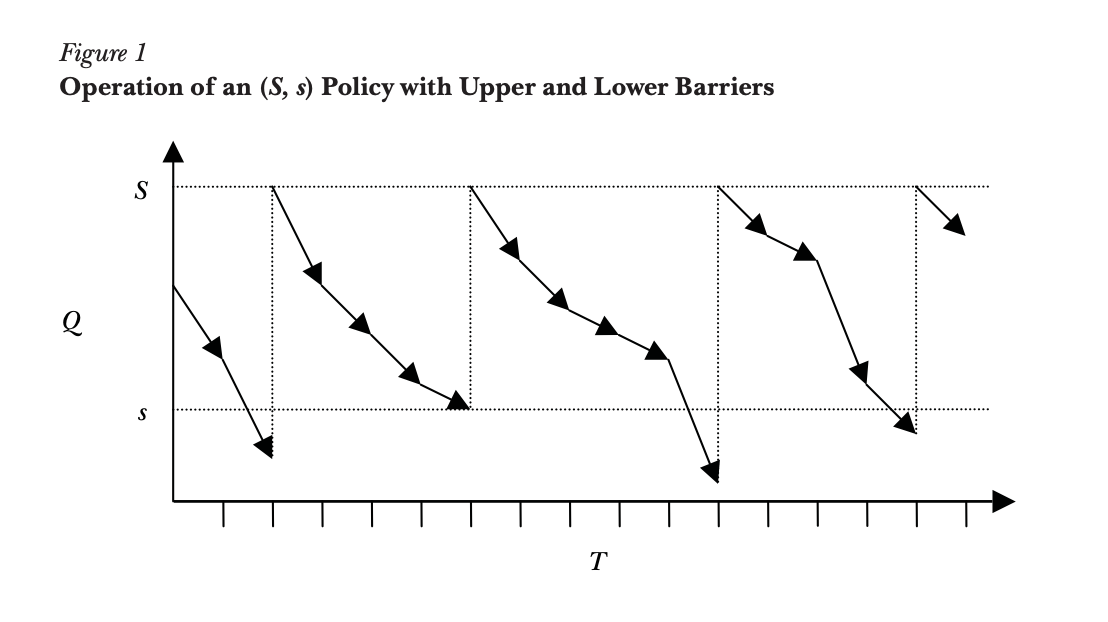
\includegraphics[scale=0.5]{FiguresTables/S_s_terminology}
\end{figure}
\end{frame}


\begin{frame}{Fixing terms - Lumpy Investment}
\begin{itemize}
\item Lumpy adjustment: Periods of no change (inaction), followed by periods of substantial change (spikes)
\pause
\item Intuitive that some investment expenditures are lumpy
\begin{itemize}
\item Example: A firm usually does not build a new factory, but sometimes it doubles the number of factories it has
\item Some may not be: maintenance
\end{itemize}
\item If too lumpy, models that imply smooth micro investment might be off
\pause
\item May reflect increasing returns in the adjustment technology
\pause
\item It may be better to invest a lot at once, rather than smooth it out
\end{itemize}
\end{frame}


\begin{frame}{Doms and Dunne (1998)}
Good example of a ``facts'' paper that reshaped a field
\begin{itemize}
\item Fundamental Question: How Lumpy is investment after all?
\item Subsequent question: What does lumpiness depend on?
\end{itemize}
\pause
Data
\begin{itemize}
\item U.S. data 1972-1988
\item LRD from the Census Bureau
\item Small sample: 13,702 establishments (of 350,000)
\item Large establishments: account for 50\% of manufacturing output
\end{itemize}
\end{frame}

\begin{frame}{Doms and Dunne (1998)}
Significant inaction
\begin{itemize}
\item In a given year, 80\% of plants change their capital stock by < 10\%
\item ... 51.9\% of plants ... by less than 2.5\%
\end{itemize}
\end{frame} 

\begin{frame}{Distribution of Investment Rates}
From Cooper and Haltwanger (2006). Same data. $I/K$. Skewed, large mass at 0, with fat tails
\begin{figure}
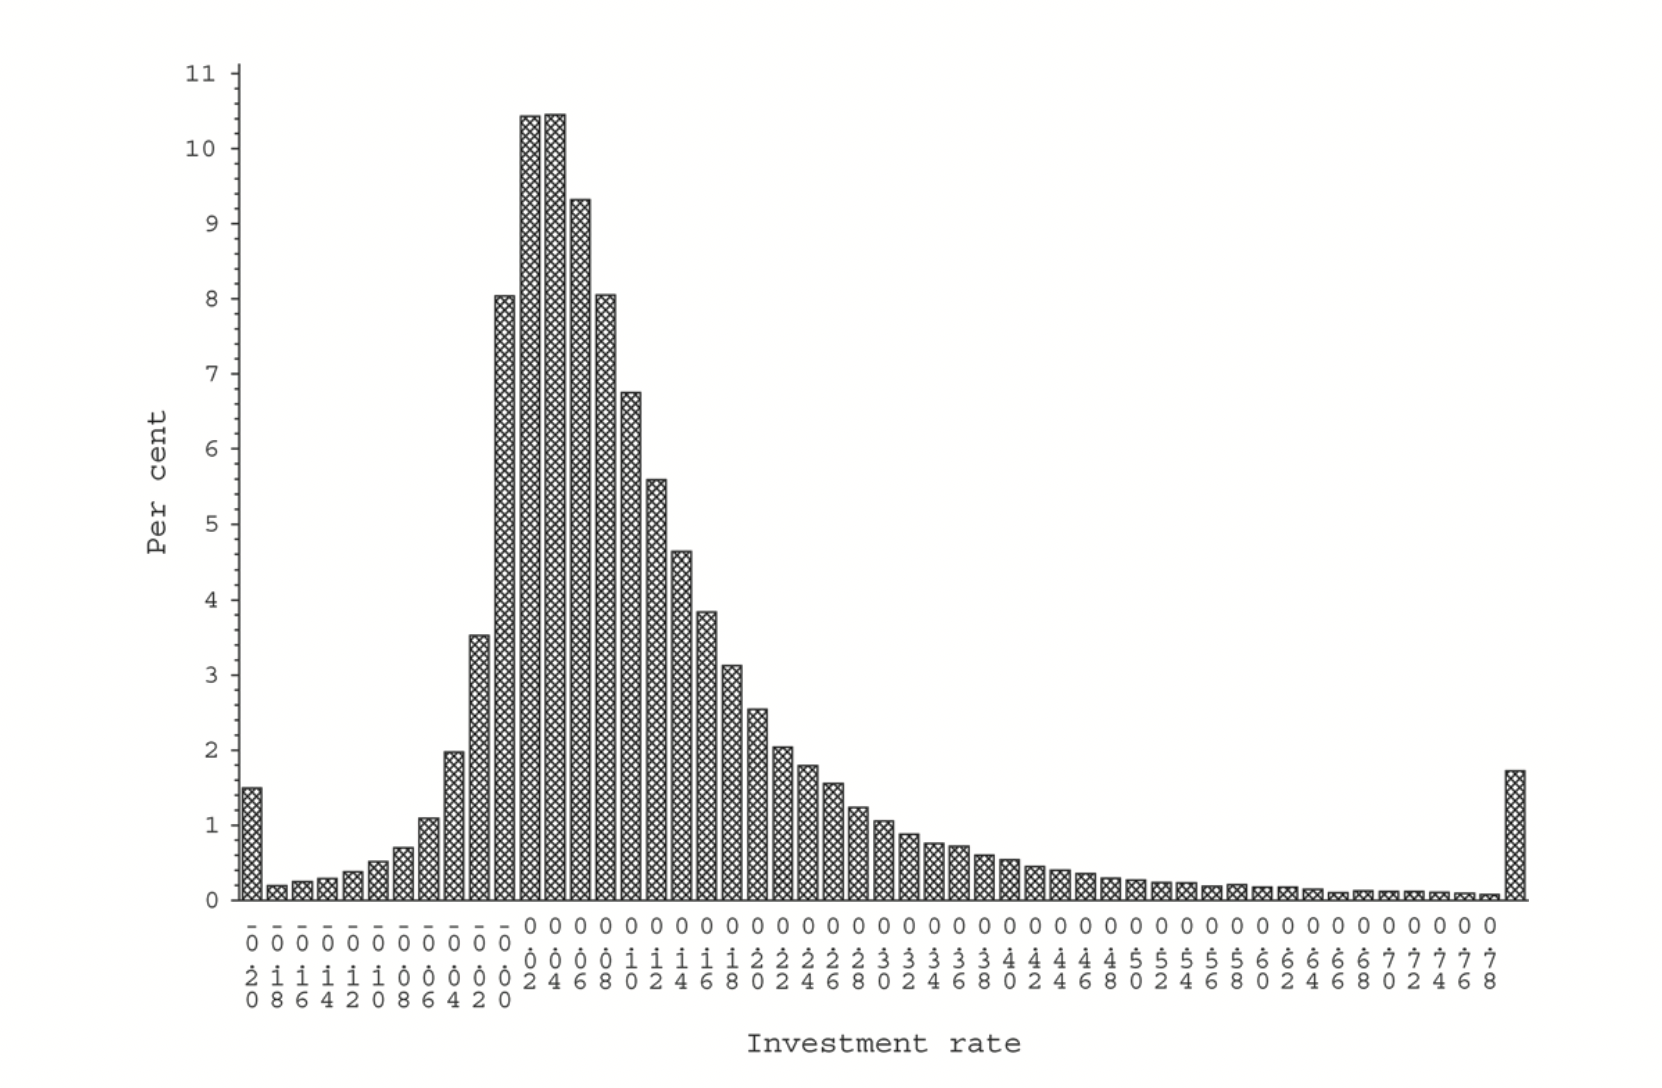
\includegraphics[scale=0.34]{FiguresTables/histogram_cooper_haltiwanger}
\end{figure}
\end{frame}



\begin{frame}{Distribution of Investment Rates}
From Cooper and Haltwanger (2006). Same data. 1972 - 1988
\begin{figure}
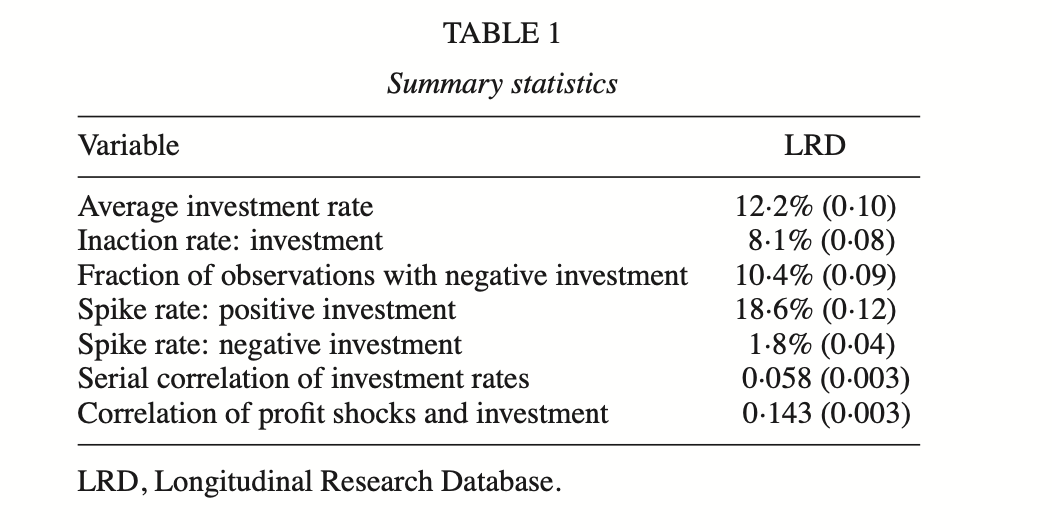
\includegraphics[scale=0.5]{FiguresTables/table_cooper_haltiwanger}
\end{figure}
Very low autocorrelation. Puzzling if you think that shocks (demand, productivity) are persistent
\end{frame}


\begin{frame}{Distribution of Investment Rates}
From Zwick and Mahon (2017). Stratified sample of tax returns. 1993 - 2010
\begin{figure}
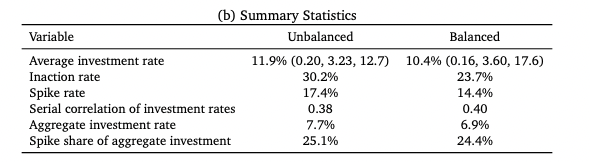
\includegraphics[scale=0.5]{FiguresTables/zwick_mahon_tab}
\end{figure}
Higher autocorrelation (Does not include structures). Higher inaction (includes smaller firms)
\end{frame}

\begin{frame}{Cross-sectional Patterns}
There is some lumpiness, but compared to what? We need some benchmark
\end{frame}

\begin{frame}{Doms and Dunne (1998)}
Define two objects
\begin{itemize}
\item Growth rate of capital $GK$ (why that formula?)
$$GK_{i,t} = \frac{I_{i,t} - \delta K_{i,t-1}}{0.5(K_{i,t} + K_{i,t-1})}$$
\pause
\item And the (within-firm) share of investment in a given year
$$\text{Investment Share}_{i,t} = \frac{I_{i,t}}{\sum_{\tau} I_{i,\tau}}$$
\end{itemize}
\end{frame}

\begin{frame}{Doms and Dunne (1998)}
\begin{figure}
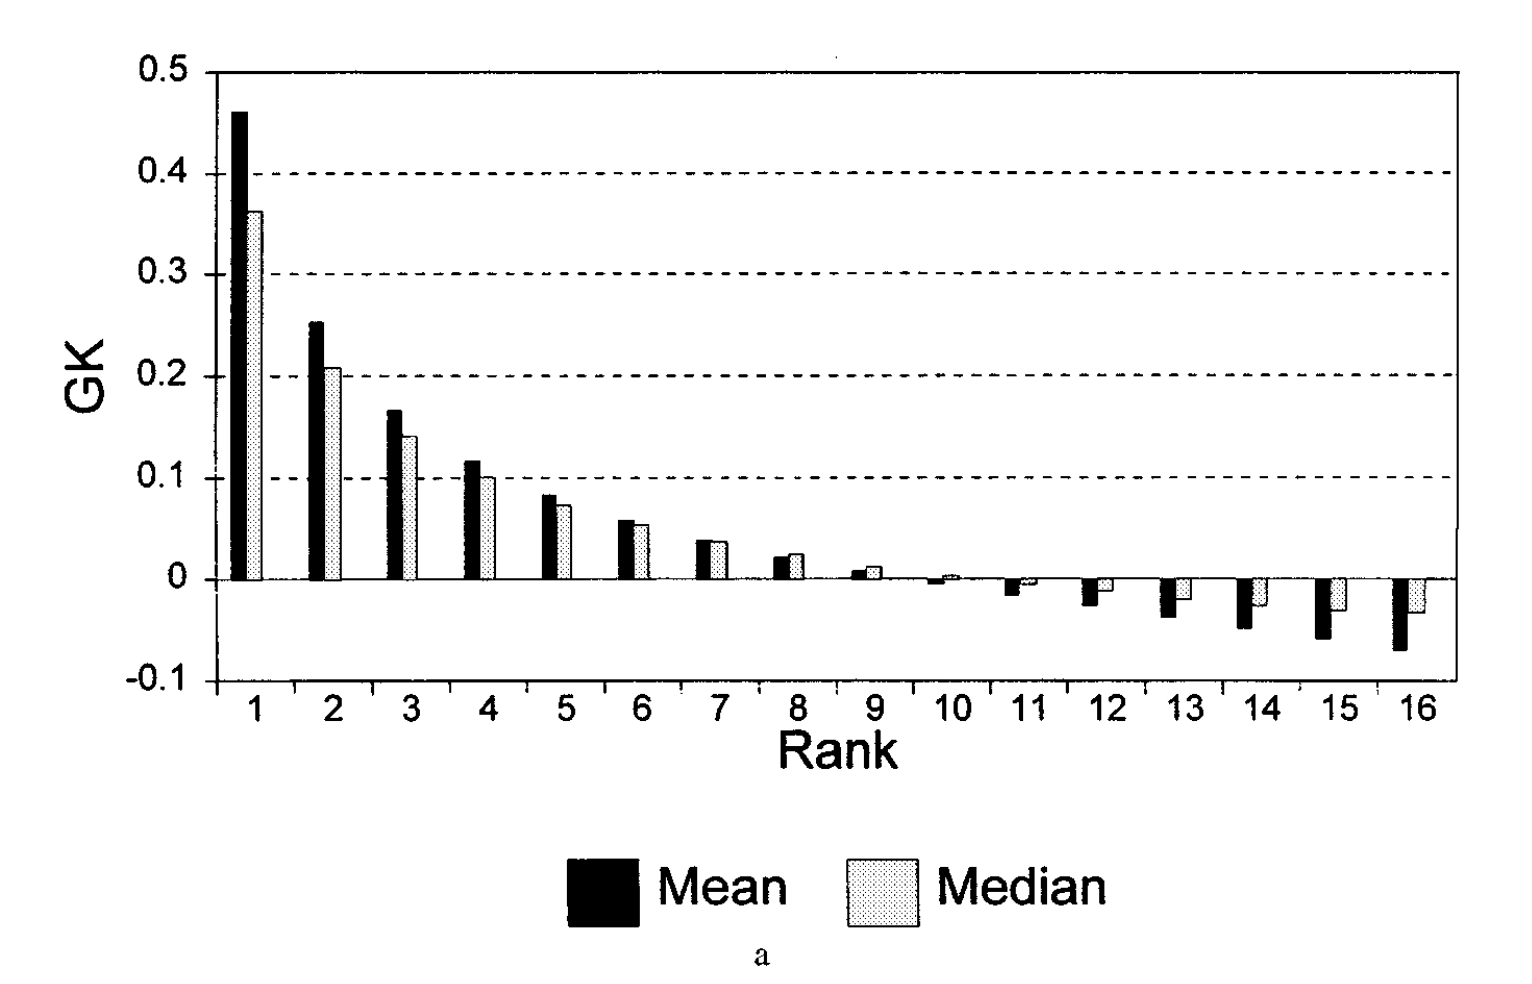
\includegraphics[scale=0.37]{FiguresTables/doms_dune_gk}
\end{figure}
Rank is the year in which $GK$ was the $n-th$ highest at the establishment level
\end{frame}

\begin{frame}{Doms and Dunne (1998)}
\begin{figure}
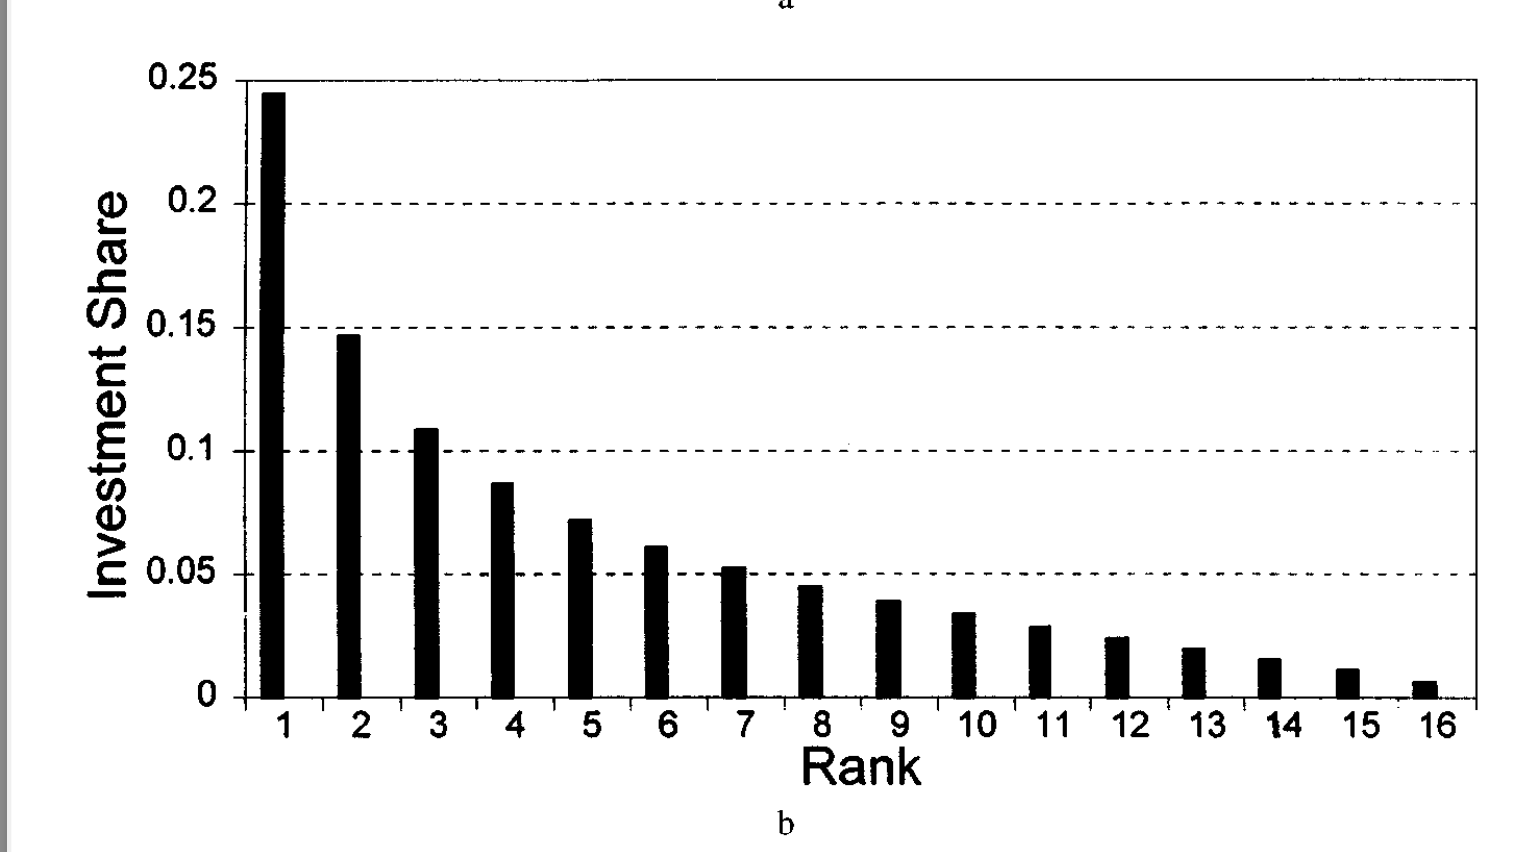
\includegraphics[scale=0.37]{FiguresTables/doms_dune_ishare}
\end{figure}
Rank is the year in which $IS$ was the $n-th$ highest at the establishment level
\end{frame}

\begin{frame}{Taking Stock}
Of course the previous two figures have decreasing patterns, duh
\begin{itemize}
\item The good question is: How fast are capital growth rates decreasing?
\end{itemize}
\pause
They propose a statistical model, which will make a comeback
\begin{itemize}
\pause
\item Define $k_{i,t}^*$ as the (log) desired level of capital at the firm
$$k_{i,t}^* = k_{i,t-1}^* + \epsilon_{i,t}$$
\item For $\epsilon$ distributed $N(\mu,\sigma)$
\pause
\item And define $z_{i,t}$ as the gap between desired and actual capital stocks
$$z_{i,t} = k_{i,t} - k_{i,t}^*$$
\end{itemize}
\end{frame}

\begin{frame}{Two views}
Imagine there are no frictions to adjust your capital stock
\pause
\begin{itemize}
\item $z_{i,t} = 0$
\pause
\item $k_{i,t} = k^*_{i,t}$ by definition
\end{itemize}
\pause
Imagine a world in which adjusting capital is ``difficult''
\begin{itemize}
\item If $z$ is too low, then adjust upward
\pause
$$ \text{if  } z_{i,t}<L \text{,  then  set } k_{i,t} \text{  such that  } z_{i,t} = l$$
\pause
\item If $z$ is too large, then adjust downward
$$ \text{if  } z_{i,t}> U \text{,  then  set } k_{i,t} \text{  such that  } z_{i,t} = u$$
\end{itemize}
\pause
For $L < l < u < U$
\end{frame}


\begin{frame}{Doms and Dunne (1998)}
\begin{figure}
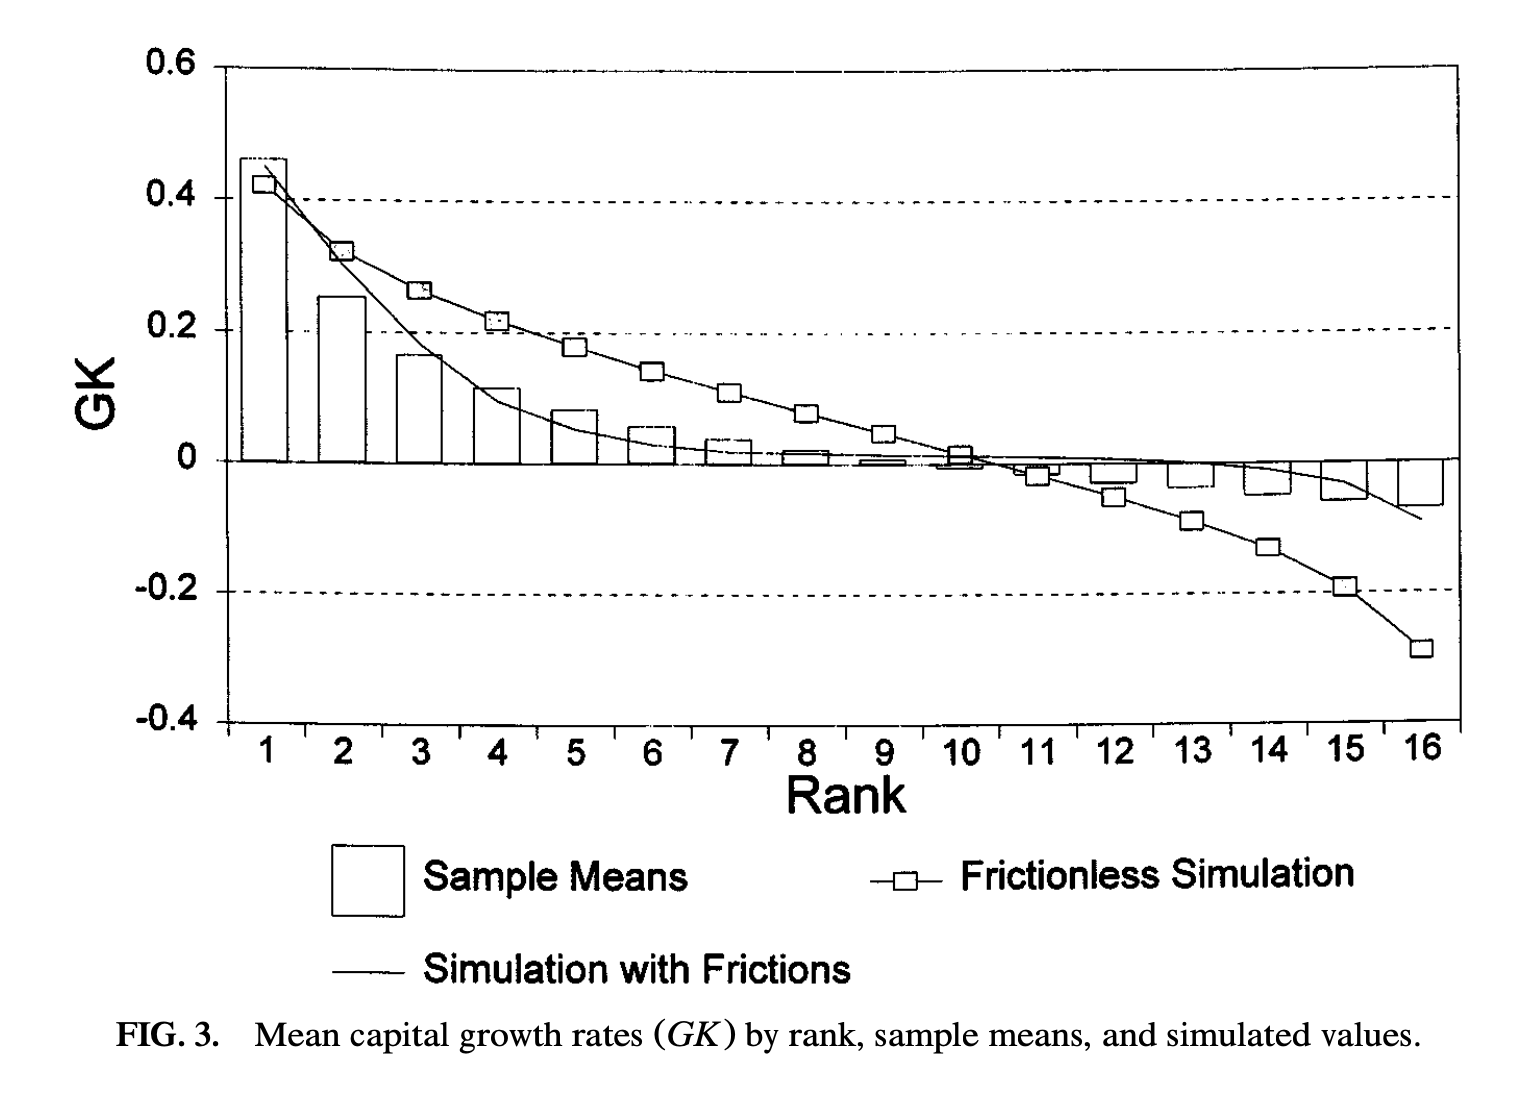
\includegraphics[scale=0.3]{FiguresTables/doms_dune_two_models}
\end{figure}
Very simple example of ``moment matching''
\end{frame}


\begin{frame}{Further Evidence on Lumpiness}
Gourio and Kashyap (2007). Can lumpiness explain aggregate investment at business cycle frequencies?
\pause
\begin{itemize}
\item Decompose investment rates $I_{t}/K_t$ into
\item $I20/K$, with investment of firms with spikes ($I_{it}/K_{it-1} > 0.2$)
\pause
\item $I(0-20)/K$, with investment of firms without spikes ($0 < I_{it}/K_{it-1} < 0.2$)
\pause
\item Data from manufacturing surveys from Chile and U.S.
\end{itemize}
\pause
Arbitrary number of decompositions you can make, some are insightful!
\end{frame}


\begin{frame}{Investment spikes appear to be important}
\begin{figure}
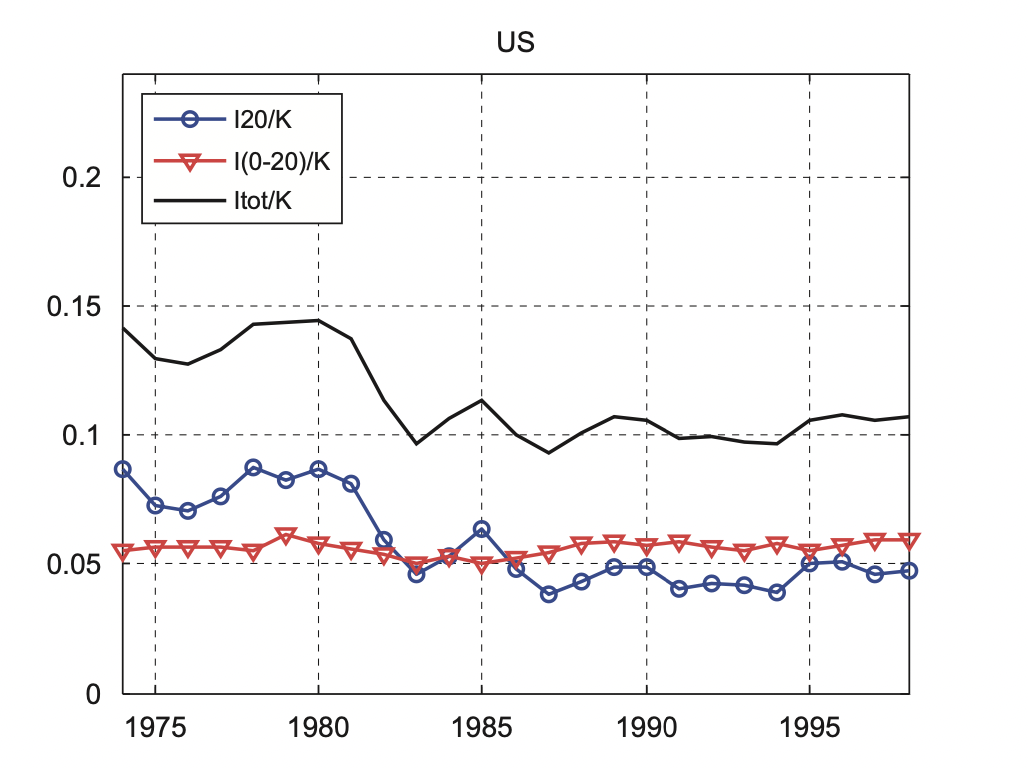
\includegraphics[scale=0.42]{FiguresTables/spikes_us}
\end{figure}
Investment rates comove with the investment rate of firms with spikes. Point at the large share.
\end{frame}

\begin{frame}{Investment spikes appear to be important}
\begin{figure}
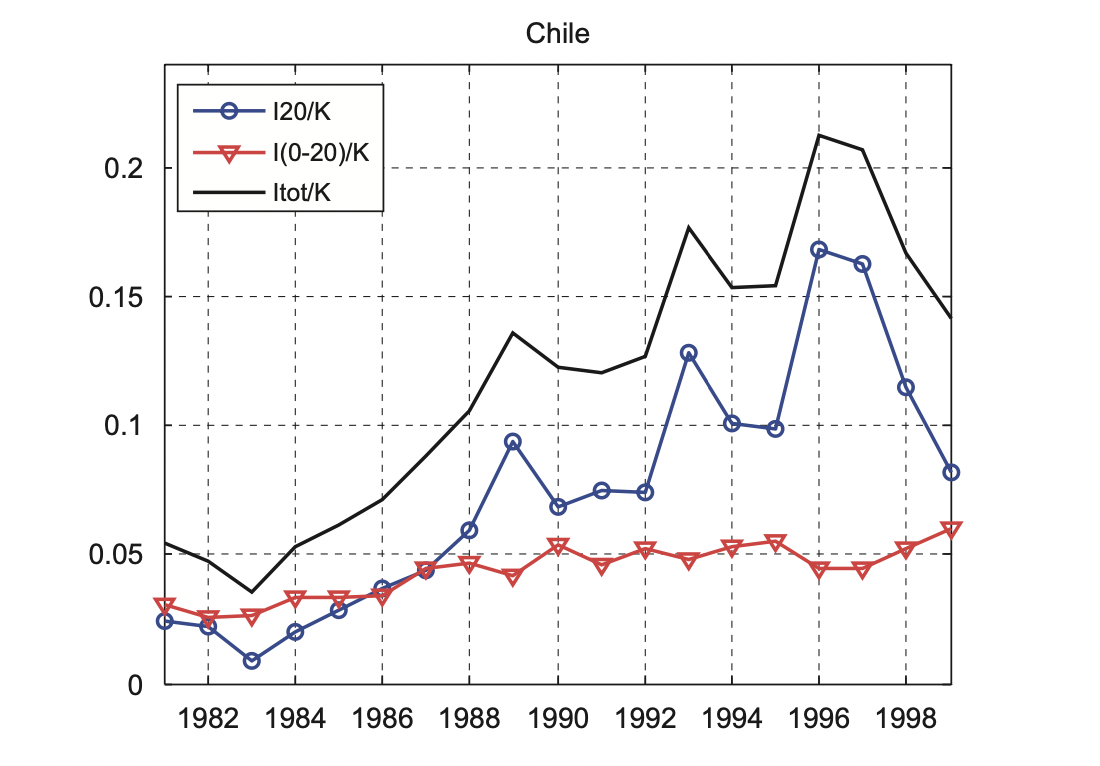
\includegraphics[scale=0.42]{FiguresTables/spikes_chile}
\end{figure}
Investment rates comove with the investment rate of firms with spikes. Point at the large share. Gourio and Kashyap (2007).
\end{frame}




\begin{frame}{Intensive vs. extensive margin}
\begin{itemize}
\item Take the share of investment happening at firms experiencing investment spikes
\begin{align}
\frac{I^{20}_t}{K_t}
\end{align}
\pause
\item Multiply and divide by the capital of firms with spikes $K^{20}$.
$$\frac{I^{20}_t}{K_t}
 = \frac{I^{20}_t}{K_t} \frac{K^{20}_t}{K^{20}_t} = \frac{I^{20}_t}{K^{20}_t} \times \frac{K^{20}_t}{K_t}$$
\pause
\item $\frac{I^{20}_t}{K^{20}_t}$ is the avg. rate at firms with spikes. The intensive margin.
\pause
\item $\frac{K^{20}_t}{K_t}$ is the (capital weighted) share of firms with spikes. The extensive margin.
$$\frac{\sum_i K_{i,t} \mathds{1}_{spike}}{\sum K_{i,t}} = \frac{\sum_{i \in spike} K_{i,t}}{K_t} = \frac{K^{20}_t}{K_t}$$
\end{itemize}
\end{frame}

\begin{frame}{Importance of the extensive margin}
\begin{figure}
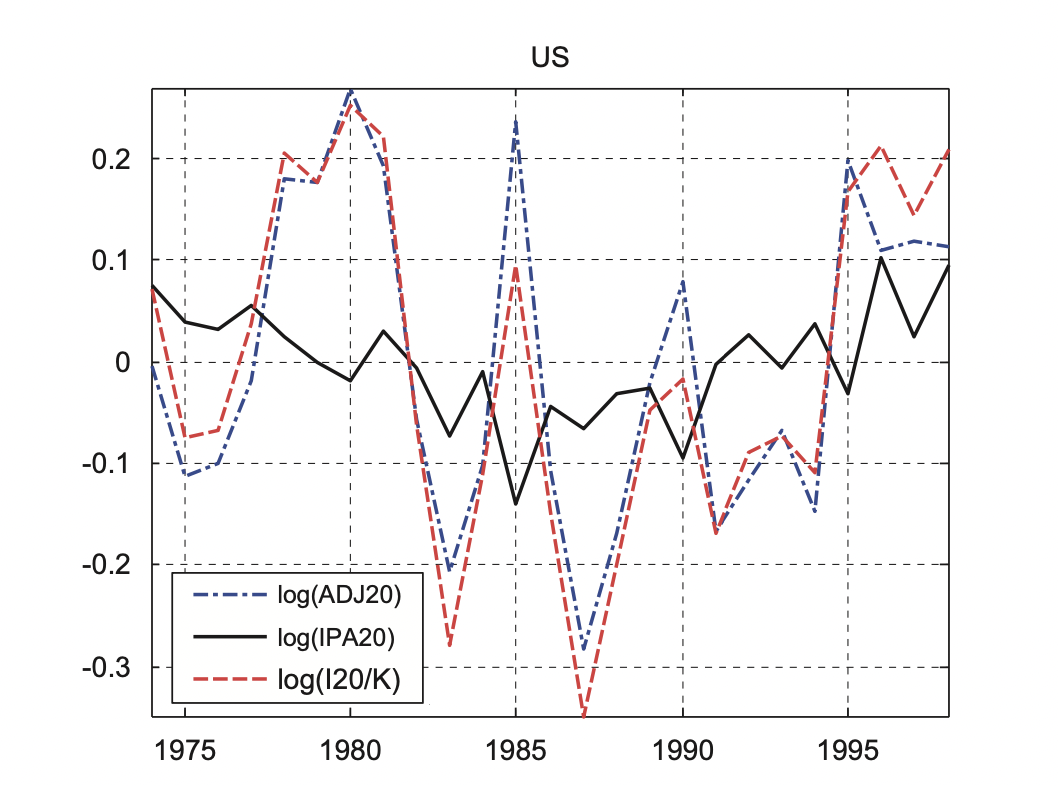
\includegraphics[scale=0.42]{FiguresTables/decomp_us}
\end{figure}
Investment rates comove with the ``extensive margin''
\end{frame}


\begin{frame}{Importance of the extensive margin}
\begin{figure}
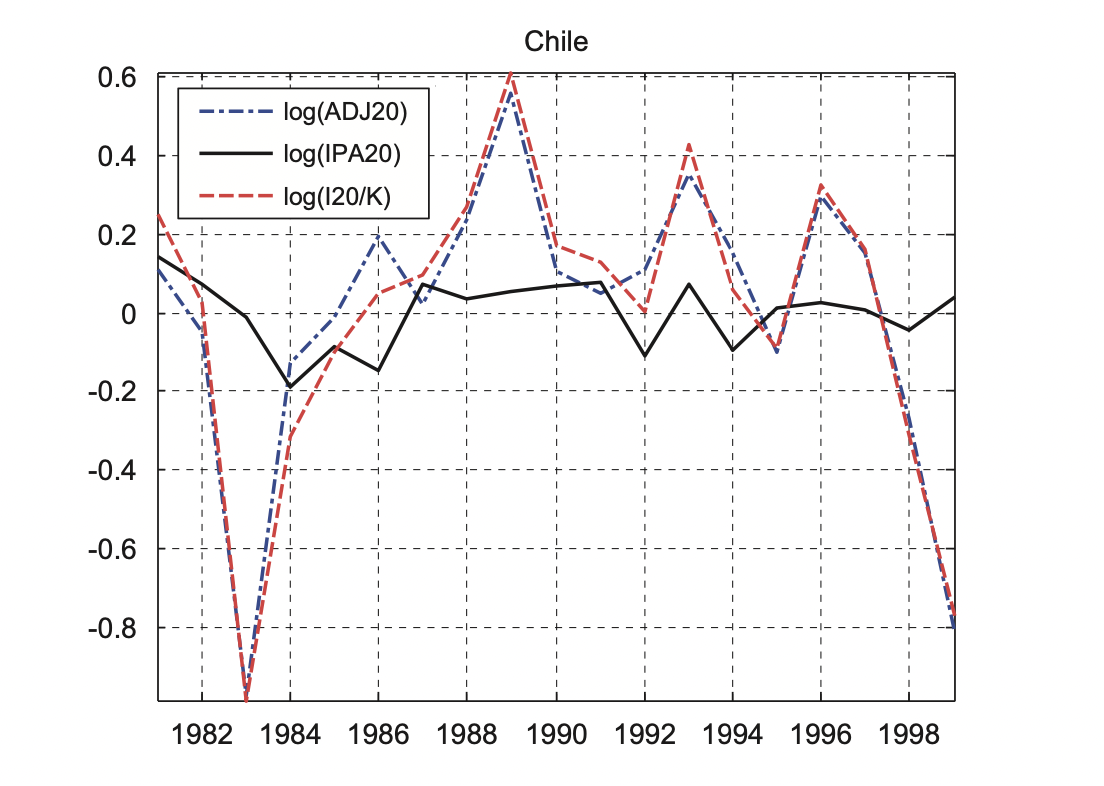
\includegraphics[scale=0.42]{FiguresTables/decomp_chile}
\end{figure}
Investment rates comove with the ``extensive margin''
\end{frame}


\begin{frame}{Firm-Level Behavior}
\begin{itemize}
\item We will start in Partial Equilibrium
\pause
\item Time is discrete
\pause
\item Firms have decreasing returns to scale (why?)
\pause
\item They sell homogeneous goods
\pause
\item They rent labor in a competitive market
\pause
\item They purchase capital
\pause
\item wages are exogenous
\pause
\item Firms discount the future with $\beta$, not the SDF of the household
\pause
\item Equivalent to the real interest rate being constant
\end{itemize}
\end{frame}

\begin{frame}{Adjustment Costs}
\begin{itemize}
\item Firms face fixed (non-convex) adjustment costs
\pause
\item In order to invest $i_{jt} \neq 0$ firms need to pay a cost $\chi_{jt}$
\item They will also face quadratic (convex) adjustment costs
\pause
\item When investing $i_{jt}$, firms pay $\frac{\psi}{2}\left(\frac{i_{jt}}{k_{jt}}\right)^2 k_{jt}$
\pause
\item We include both due to evidence in Cooper and Haltiwanger (2006)
\pause
\item We covered some figures of that paper but we will take another look
\end{itemize}
\end{frame}


\begin{frame}{Profits}
\begin{itemize}
\item Firm profits are given by:
$$\pi_{jt} = a_{jt} k^{\theta}_{jt} l_{jt}^{\nu} - w_t l_{jt} - w_t \chi_{jt}\mathds{1}_{i_{jt} \neq 0} -  \frac{\psi}{2}\left(\frac{i_{jt}}{k_{jt}}\right)^2 k_{jt}$$
\vspace{-0.5cm}
\pause
\item Decreasing returns to scale give a well-defined firm distribution
\pause
\item We could have done CRS in production and downward sloping demand curves
\pause
\item Note that we are denoting the fixed costs in units of labor. You need to devote $\chi_{jt}$ workers in order to come-up with an investment plan
\pause
\item  $\chi_{jt}$ are fixed costs of adjustment. Constant conditional on adjustment, and zero in the case of inaction
\pause
\item Including $\chi$ and $\psi$ is without loss. We could plausibly set them to zero
\item Similar to the Golosov Lucas (2007) model but for capital
\end{itemize}
\end{frame}

\begin{frame}{Firm's Problem}
\begin{itemize}
\item Firms maximize firm value
$$V(k_j,a_j) = \max_{l_j} \left\lbrace a_{jt} k^{\theta}_{j} l_{j}^{\nu} - w_t l_{j} \right\rbrace + \max \left\lbrace V^n(k_j,a_j), V^a(k_j,a_j) - \chi_j w \right\rbrace $$
\vspace{-0.5cm}
\pause
\item The non-convexity introduces a discrete choice. Invest or not.
\pause
\item These are captured in the value functions $V^n$ ($n$ for no), and  $V^a$ ($a$ for adjustment).
\pause
\item Note that labor demand is a static choice, so labor is not a state variable
\pause
\item We now need to specify what $V^n$ and $V^a$ look like
\end{itemize}
\end{frame}


\begin{frame}{The value of non-adjusting}
\begin{itemize}
\item Firms maximize firm value
$$V(k_j,a_j) = \max_{l_j} \left\lbrace a_{jt} k^{\theta}_{j} l_{j}^{\nu} - w_t l_{j} \right\rbrace + \max \left\lbrace V^n(k_j,a_j), V^a(k_j,a_j) - \chi_j w \right\rbrace $$
\vspace{-0.5cm}
\item The value function in case of not-adjusting is
$$V^n(k_j,a_j) = \beta \mathbb{E} \left[ V(k'_j, a'_j) | a_j \right]$$
\vspace{-0.5cm}
\item subject to
$$k_j' = (1-\delta) k_j$$
\end{itemize}
\end{frame}

\begin{frame}{The value of adjusting}
\begin{itemize}
\item Firms maximize firm value
$$V(k_j,a_j) = \max_{l_j} \left\lbrace a_{jt} k^{\theta}_{j} l_{j}^{\nu} - w_t l_{j} \right\rbrace + \max \left\lbrace V^n(k_j,a_j), V^a(k_j,a_j) - \chi_j w \right\rbrace $$
\item The value function in case of adjusting is
$$V^a(k_j,a_j) =\max_{i_j} \left\lbrace- i  - \frac{\psi}{2}\left(\frac{i_{jt}}{k_{jt}}\right)^2 k_{j} + \beta \mathbb{E} \left[ V(k'_j, a'_j) | a_j \right] \right\rbrace$$
\vspace{-0.5cm}
\item subject to
$$k_j' = (1-\delta) k_j + i_j $$
\pause
\item We will assume that $\chi_j$ is iid across firms, and
$$\chi_j \sim U[\underline{\chi},\bar{\chi}]$$
\end{itemize}
\end{frame}

\begin{frame}{Firm's Problem}
\begin{itemize}
\item Firms maximize firm value
$$V(k_j,a_j) = \max_{l_j} \left\lbrace a_{jt} k^{\theta}_{j} l_{j}^{\nu} - w_t l_{j} \right\rbrace + \max \left\lbrace V^n(k_j,a_j), V^a(k_j,a_j) - \chi_j w \right\rbrace $$
\item The value function in case of not-adjusting is
$$V^n(k_j,a_j) = \beta \mathbb{E} \left[ V(k'_j, a'_j) | a_j \right]$$
\vspace{-0.5cm}
$$k_j' = (1-\delta) k_j$$
\vspace{-0.5cm}
\item The value function in case of adjusting is
$$V^a(k_j,a_j) =\max_{i_j} \left\lbrace- i  - \frac{\psi}{2}\left(\frac{i_{jt}}{k_{jt}}\right)^2 k_{j} + \beta \mathbb{E} \left[ V(k'_j, a'_j) | a_j \right] \right\rbrace$$
\vspace{-0.5cm}
$$k_j' = (1-\delta) k_j + i_j $$
\vspace{-0.5cm}
\end{itemize}
\end{frame}

\begin{frame}{The easy part - labor demand}
\begin{itemize}
\item Labor demand is almost trivial in this model
\pause
\item Capital is fixed within the period
\pause
\item The first order condition is just
$$l(k_j,a_j) = \left(\frac{\nu a_j k_j^{\theta}}{w}\right)^{\frac{1}{1-\nu}} $$
\end{itemize}
\end{frame}

\begin{frame}{The decision of adjusting}
\begin{itemize}
\item Simple: you adjust if it is worth it
$$\text{adjust iff  }  V^a(k_j,a_j)  - \chi w > V^n(k_j,a_j)$$
\item Which implies an upper threshold for adjustment
$$\hat{\chi}(k_j,a_j) =  \frac{V^a(k_j,a_j)  - V^n(k_j,a_j)}{w}  $$
\pause
\item Adjustment iff $\chi_j < \hat{\chi}(k_j,a_j)$
\item So we can compute a probability of adjustment: The probability that a firm with state $k,a$ adjusts it's capital stock
\pause
$$P(\chi_j < \hat{\chi}(k_j,a_j)) = \frac{\hat{\chi}(k_j,a_j) - \underline{\chi}}{\bar{\chi} - \underline{\chi}}$$
\end{itemize}
\end{frame}

\begin{frame}{Individual level adjustment decision}
\begin{itemize}
\item At the individual level adjustment is random
\pause
\item And we can compute probabilities of adjustment in the state-space
\pause
\item Why did we pick this assumptions?
\begin{itemize}
\item We want to have a simple model that allows for periods of inaction
\pause
\item Recognize that similar firms sometimes adjust and sometimes do not
\pause
\item In this sense, variation in $\chi$ is a reduced form way of capturing our ignorance
\pause
\item Stuff we do not understand that drives the decision to adjust at one time or another
\end{itemize}
\end{itemize}
\end{frame}

\begin{frame}{Investment Conditional on adjustment}
\begin{itemize}
\item The value function in case of adjusting is
$$V^a(k_j,a_j) =\max_{i_j} \left\lbrace- i  - \frac{\psi}{2}\left(\frac{i_{jt}}{k_{jt}}\right)^2 k_{j} + \beta \mathbb{E} \left[ V(k'_j, a'_j) | a_j \right] \right\rbrace$$
\vspace{-0.5cm}
$$k_j' = (1-\delta) k_j + i_j $$
\vspace{-0.5cm}
\pause
\item With first order condition
$$\frac{i_j}{k_j} = \frac{\beta \mathbb{E}  \left[ V_k(k_j',a_j')|a_j \right] - 1}{\psi}$$
\pause
\item Notice that conditional on adjustment investment has a $q$ flavor
\pause
\item Not a coincidence, we extended the framework to:
\begin{itemize}
\item Heterogeneous firms
\item Idiosyncratic shocks
\item non-convex costs
\end{itemize}
\end{itemize}
\end{frame}

\begin{frame}{Intuition of the Problem}
\begin{itemize}
\item Let's turn to a simplified problem of a firm with profit function
$$\Pi(k,a) = ak^{\beta} - (\delta + r) k$$
\pause
\item And only random fixed costs of adjustment
\item Without convex costs  ($\psi =0$)
\pause
\item This is the framework of Caballero and Engel (1999) in your required readings
\end{itemize}
\end{frame}

\begin{frame}{Intuition of the Problem}


\tikzset{every picture/.style={line width=0.75pt}} %set default line width to 0.75pt        

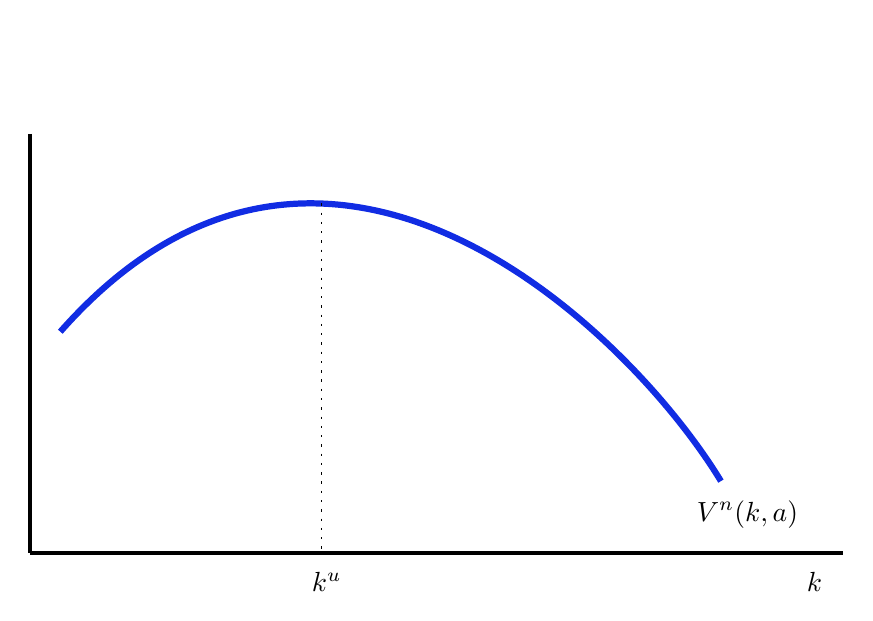
\begin{tikzpicture}[x=0.75pt,y=0.75pt,yscale=-0.7,xscale=0.7]
%uncomment if require: \path (0,341); %set diagram left start at 0, and has height of 341

%Straight Lines [id:da9871078943096634] 
\draw [line width=1.5]    (82.11,296.24) -- (642,296.24) ;
%Straight Lines [id:da14269884069755578] 
\draw [line width=1.5]    (82.11,8) -- (82.11,296.24) ;
%Curve Lines [id:da27890825471441794] 
\draw [color={rgb, 255:red, 17; green, 44; blue, 227 }  ,draw opacity=1 ][line width=2.25]    (103.15,144.15) .. controls (286,-62.97) and (496.36,145.6) .. (557.85,246.99) ;
%Straight Lines [id:da08627712735151372] 
\draw  [dash pattern={on 0.84pt off 2.51pt}]  (282.76,55.8) -- (282.76,294.79) ;

% Text Node
\draw (615.27,307.69) node [anchor=north west][inner sep=0.75pt]    {$k$};
% Text Node
\draw (539.51,258.35) node [anchor=north west][inner sep=0.75pt]    {$V^{n}( k,a)$};
% Text Node
\draw (274.45,307.69) node [anchor=north west][inner sep=0.75pt]    {$k^{u}$};


\end{tikzpicture}
\end{frame}

\begin{frame}{Intuition of the Problem}

\tikzset{every picture/.style={line width=0.75pt}} %set default line width to 0.75pt        

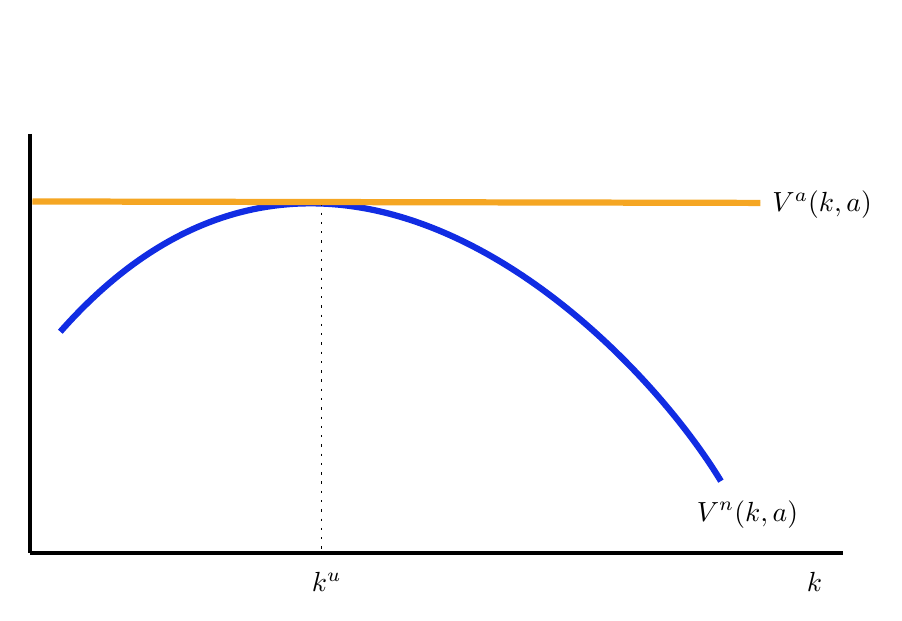
\begin{tikzpicture}[x=0.75pt,y=0.75pt,yscale=-0.7,xscale=0.7]
%uncomment if require: \path (0,341); %set diagram left start at 0, and has height of 341

%Straight Lines [id:da3568280180329646] 
\draw [line width=1.5]    (82.11,296.24) -- (642,296.24) ;
%Straight Lines [id:da7638994079892822] 
\draw [line width=1.5]    (82.11,8) -- (82.11,296.24) ;
%Curve Lines [id:da2971453465398075] 
\draw [color={rgb, 255:red, 17; green, 44; blue, 227 }  ,draw opacity=1 ][line width=2.25]    (103.15,144.15) .. controls (286,-62.97) and (496.36,145.6) .. (557.85,246.99) ;
%Straight Lines [id:da8380178627982076] 
\draw  [dash pattern={on 0.84pt off 2.51pt}]  (282.76,55.8) -- (282.76,294.79) ;
%Straight Lines [id:da310665362049553] 
\draw [color={rgb, 255:red, 245; green, 166; blue, 35 }  ,draw opacity=1 ][fill={rgb, 255:red, 217; green, 147; blue, 31 }  ,fill opacity=1 ][line width=2.25]    (84,54.5) -- (585,55.5) ;

% Text Node
\draw (615.27,307.69) node [anchor=north west][inner sep=0.75pt]    {$k$};
% Text Node
\draw (539.51,258.35) node [anchor=north west][inner sep=0.75pt]    {$V^{n}( k,a)$};
% Text Node
\draw (274.45,307.69) node [anchor=north west][inner sep=0.75pt]    {$k^{u}$};
% Text Node
\draw (591.51,45.35) node [anchor=north west][inner sep=0.75pt]    {$V^{a}( k,a)$};
\end{tikzpicture}
\end{frame}

\begin{frame}


\tikzset{every picture/.style={line width=0.75pt}} %set default line width to 0.75pt        

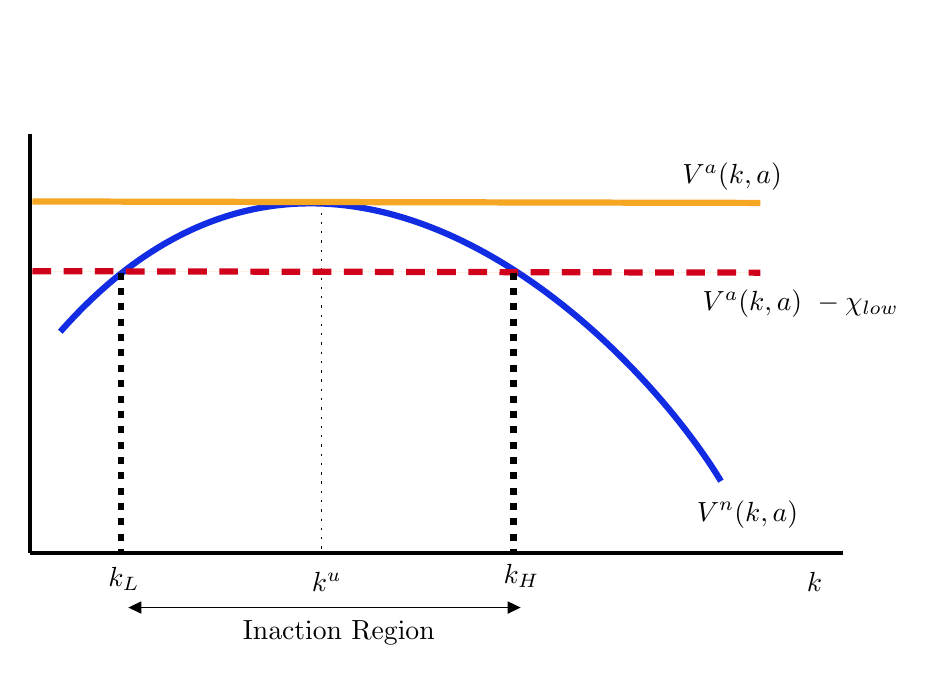
\begin{tikzpicture}[x=0.75pt,y=0.75pt,yscale=-0.7,xscale=0.7]
%uncomment if require: \path (0,365); %set diagram left start at 0, and has height of 365

%Straight Lines [id:da25182918672552645] 
\draw [line width=1.5]    (82.11,296.24) -- (642,296.24) ;
%Straight Lines [id:da9761023145284824] 
\draw [line width=1.5]    (82.11,8) -- (82.11,296.24) ;
%Curve Lines [id:da2979361963587117] 
\draw [color={rgb, 255:red, 17; green, 44; blue, 227 }  ,draw opacity=1 ][line width=2.25]    (103.15,144.15) .. controls (286,-62.97) and (496.36,145.6) .. (557.85,246.99) ;
%Straight Lines [id:da3669488319799088] 
\draw  [dash pattern={on 0.84pt off 2.51pt}]  (282.76,55.8) -- (282.76,294.79) ;
%Straight Lines [id:da6366665006085808] 
\draw [color={rgb, 255:red, 245; green, 166; blue, 35 }  ,draw opacity=1 ][fill={rgb, 255:red, 217; green, 147; blue, 31 }  ,fill opacity=1 ][line width=2.25]    (84,54.5) -- (585,55.5) ;
%Straight Lines [id:da4103521519215174] 
\draw [color={rgb, 255:red, 208; green, 2; blue, 27 }  ,draw opacity=1 ][fill={rgb, 255:red, 217; green, 147; blue, 31 }  ,fill opacity=1 ][line width=2.25]  [dash pattern={on 6.75pt off 4.5pt}]  (84,102.5) -- (585,103.5) ;
%Straight Lines [id:da522245582664139] 
\draw [line width=2.25]  [dash pattern={on 2.53pt off 3.02pt}]  (145,103.5) -- (145,296.5) ;
%Straight Lines [id:da3004255350928513] 
\draw [line width=2.25]  [dash pattern={on 2.53pt off 3.02pt}]  (415,103.5) -- (415,296.5) ;
%Straight Lines [id:da696243864407972] 
\draw    (153,334) -- (417,334) ;
\draw [shift={(420,334)}, rotate = 180] [fill={rgb, 255:red, 0; green, 0; blue, 0 }  ][line width=0.08]  [draw opacity=0] (8.93,-4.29) -- (0,0) -- (8.93,4.29) -- cycle    ;
\draw [shift={(150,334)}, rotate = 0] [fill={rgb, 255:red, 0; green, 0; blue, 0 }  ][line width=0.08]  [draw opacity=0] (8.93,-4.29) -- (0,0) -- (8.93,4.29) -- cycle    ;

% Text Node
\draw (615.27,307.69) node [anchor=north west][inner sep=0.75pt]    {$k$};
% Text Node
\draw (539.51,258.35) node [anchor=north west][inner sep=0.75pt]    {$V^{n}( k,a)$};
% Text Node
\draw (274.45,307.69) node [anchor=north west][inner sep=0.75pt]    {$k^{u}$};
% Text Node
\draw (529.51,26.35) node [anchor=north west][inner sep=0.75pt]    {$V^{a}( k,a)$};
% Text Node
\draw (543.51,113.35) node [anchor=north west][inner sep=0.75pt]    {$V^{a}( k,a) \ -\chi _{low} \ $};
% Text Node
\draw (134.45,304.4) node [anchor=north west][inner sep=0.75pt]    {$k_{L}$};
% Text Node
\draw (406.45,302.4) node [anchor=north west][inner sep=0.75pt]    {$k_{H}$};
% Text Node
\draw (227,341) node [anchor=north west][inner sep=0.75pt]   [align=left] {Inaction Region};

\end{tikzpicture}
\end{frame}



\begin{frame}


\tikzset{every picture/.style={line width=0.75pt}} %set default line width to 0.75pt        

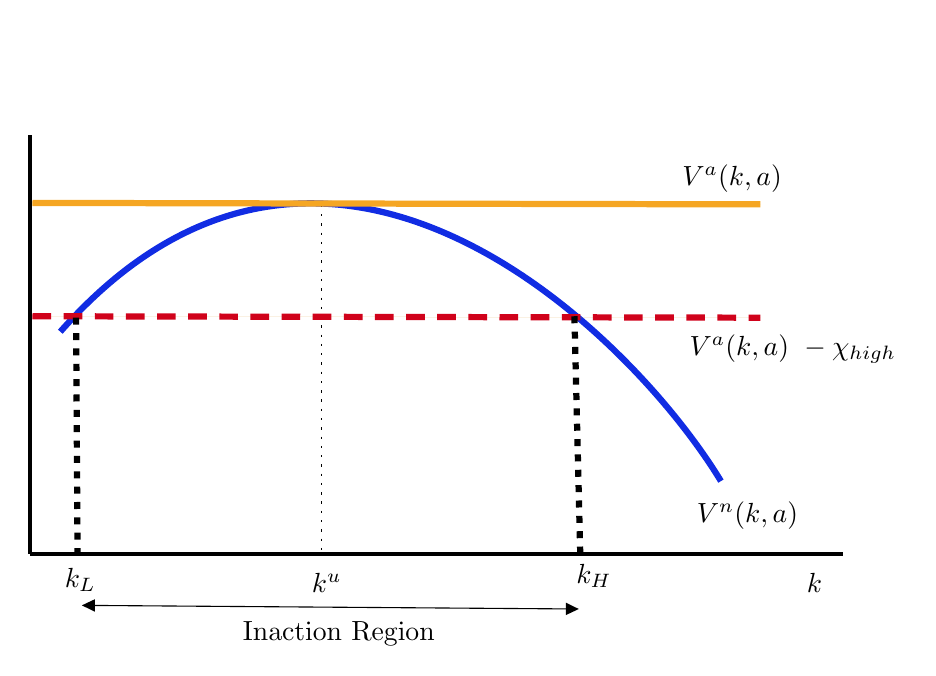
\begin{tikzpicture}[x=0.75pt,y=0.75pt,yscale=-0.7,xscale=0.7]
%uncomment if require: \path (0,365); %set diagram left start at 0, and has height of 365

%Straight Lines [id:da8073793632194175] 
\draw [line width=1.5]    (82.11,296.24) -- (642,296.24) ;
%Straight Lines [id:da8884239060649992] 
\draw [line width=1.5]    (82.11,8) -- (82.11,296.24) ;
%Curve Lines [id:da40328673035046214] 
\draw [color={rgb, 255:red, 17; green, 44; blue, 227 }  ,draw opacity=1 ][line width=2.25]    (103.15,143.15) .. controls (286,-63.97) and (496.36,144.6) .. (557.85,245.99) ;
%Straight Lines [id:da24268802741968942] 
\draw  [dash pattern={on 0.84pt off 2.51pt}]  (282.76,55.8) -- (282.76,294.79) ;
%Straight Lines [id:da04729251052493866] 
\draw [color={rgb, 255:red, 245; green, 166; blue, 35 }  ,draw opacity=1 ][fill={rgb, 255:red, 217; green, 147; blue, 31 }  ,fill opacity=1 ][line width=2.25]    (84,54.5) -- (585,55.5) ;
%Straight Lines [id:da44869414013753506] 
\draw [color={rgb, 255:red, 208; green, 2; blue, 27 }  ,draw opacity=1 ][fill={rgb, 255:red, 217; green, 147; blue, 31 }  ,fill opacity=1 ][line width=2.25]  [dash pattern={on 6.75pt off 4.5pt}]  (84,132.5) -- (585,133.5) ;
%Straight Lines [id:da46907019932769844] 
\draw [line width=2.25]  [dash pattern={on 2.53pt off 3.02pt}]  (114,133.5) -- (115,295.5) ;
%Straight Lines [id:da4004565981689805] 
\draw [line width=2.25]  [dash pattern={on 2.53pt off 3.02pt}]  (457,132.5) -- (461,295.5) ;
%Straight Lines [id:da32614127450028074] 
\draw    (121,331.52) -- (457,333.98) ;
\draw [shift={(460,334)}, rotate = 180.42] [fill={rgb, 255:red, 0; green, 0; blue, 0 }  ][line width=0.08]  [draw opacity=0] (8.93,-4.29) -- (0,0) -- (8.93,4.29) -- cycle    ;
\draw [shift={(118,331.5)}, rotate = 0.42] [fill={rgb, 255:red, 0; green, 0; blue, 0 }  ][line width=0.08]  [draw opacity=0] (8.93,-4.29) -- (0,0) -- (8.93,4.29) -- cycle    ;

% Text Node
\draw (615.27,307.69) node [anchor=north west][inner sep=0.75pt]    {$k$};
% Text Node
\draw (539.51,258.35) node [anchor=north west][inner sep=0.75pt]    {$V^{n}( k,a)$};
% Text Node
\draw (274.45,307.69) node [anchor=north west][inner sep=0.75pt]    {$k^{u}$};
% Text Node
\draw (529.51,26.35) node [anchor=north west][inner sep=0.75pt]    {$V^{a}( k,a)$};
% Text Node
\draw (534.51,143.35) node [anchor=north west][inner sep=0.75pt]    {$V^{a}( k,a) \ -\chi _{high} \ $};
% Text Node
\draw (104.45,304.4) node [anchor=north west][inner sep=0.75pt]    {$k_{L}$};
% Text Node
\draw (456.45,301.4) node [anchor=north west][inner sep=0.75pt]    {$k_{H}$};
% Text Node
\draw (227,341) node [anchor=north west][inner sep=0.75pt]   [align=left] {Inaction Region};
\end{tikzpicture}
\end{frame}

\begin{frame}{Adjustment for high $\chi$}


\tikzset{every picture/.style={line width=0.75pt}} %set default line width to 0.75pt        

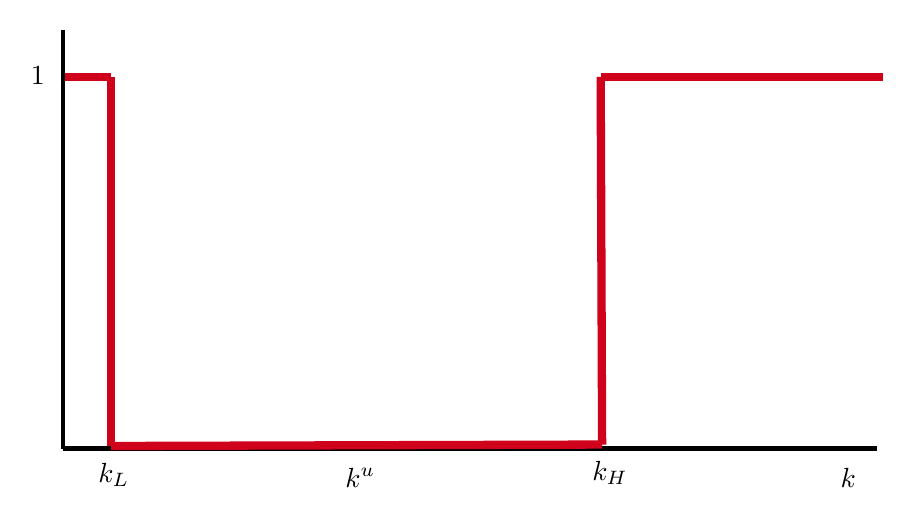
\begin{tikzpicture}[x=0.75pt,y=0.75pt,yscale=-0.7,xscale=0.7]
%uncomment if require: \path (0,365); %set diagram left start at 0, and has height of 365

%Straight Lines [id:da676461687487593] 
\draw [line width=1.5]    (82.11,296.24) -- (642,296.24) ;
%Straight Lines [id:da18506869242495938] 
\draw [line width=1.5]    (82.11,8) -- (82.11,296.24) ;
%Straight Lines [id:da8739754534014852] 
\draw [color={rgb, 255:red, 208; green, 2; blue, 27 }  ,draw opacity=1 ][line width=3]    (115,40.5) -- (115,294.5) ;
%Straight Lines [id:da5424117107486859] 
\draw [color={rgb, 255:red, 208; green, 2; blue, 27 }  ,draw opacity=1 ][line width=3]    (452,40.5) -- (453,293.5) ;
%Straight Lines [id:da5856869260155171] 
\draw [color={rgb, 255:red, 208; green, 2; blue, 27 }  ,draw opacity=1 ][line width=3]    (115,40.5) -- (83,40.5) ;
%Straight Lines [id:da062425919937421304] 
\draw [color={rgb, 255:red, 208; green, 2; blue, 27 }  ,draw opacity=1 ][line width=3]    (646,40.5) -- (452,40.5) ;
%Straight Lines [id:da5907024155632177] 
\draw [color={rgb, 255:red, 208; green, 2; blue, 27 }  ,draw opacity=1 ][line width=3]    (453,293.5) -- (115,294.5) ;

% Text Node
\draw (615.27,307.69) node [anchor=north west][inner sep=0.75pt]    {$k$};
% Text Node
\draw (274.45,307.69) node [anchor=north west][inner sep=0.75pt]    {$k^{u}$};
% Text Node
\draw (104.45,304.4) node [anchor=north west][inner sep=0.75pt]    {$k_{L}$};
% Text Node
\draw (444.45,303.4) node [anchor=north west][inner sep=0.75pt]    {$k_{H}$};
% Text Node
\draw (58,31.4) node [anchor=north west][inner sep=0.75pt]    {$1$};


\end{tikzpicture}
\end{frame}


\begin{frame}{Adjustment for mid $\chi$}


\tikzset{every picture/.style={line width=0.75pt}} %set default line width to 0.75pt        

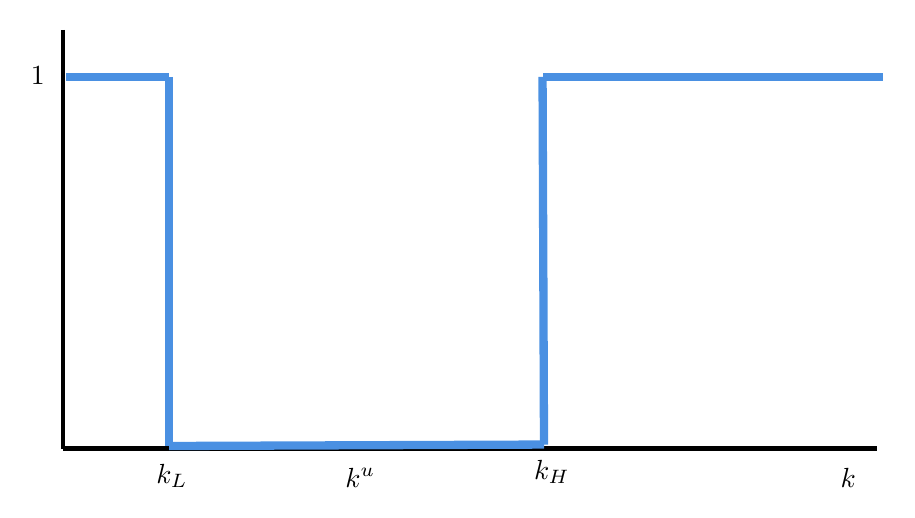
\begin{tikzpicture}[x=0.75pt,y=0.75pt,yscale=-0.7,xscale=0.7]
%uncomment if require: \path (0,365); %set diagram left start at 0, and has height of 365

%Straight Lines [id:da40163986736813406] 
\draw [line width=1.5]    (82.11,296.24) -- (642,296.24) ;
%Straight Lines [id:da8334250728349588] 
\draw [line width=1.5]    (82.11,8) -- (82.11,296.24) ;
%Straight Lines [id:da5582158851573467] 
\draw [color={rgb, 255:red, 74; green, 144; blue, 226 }  ,draw opacity=1 ][line width=3]    (155,40.5) -- (155,294.5) ;
%Straight Lines [id:da80152876235062] 
\draw [color={rgb, 255:red, 74; green, 144; blue, 226 }  ,draw opacity=1 ][line width=3]    (412,40.5) -- (413,293.5) ;
%Straight Lines [id:da8074271145240712] 
\draw [color={rgb, 255:red, 74; green, 144; blue, 226 }  ,draw opacity=1 ][line width=3]    (155,40.5) -- (84,40.5) ;
%Straight Lines [id:da2981057538779577] 
\draw [color={rgb, 255:red, 74; green, 144; blue, 226 }  ,draw opacity=1 ][line width=3]    (646,40.5) -- (412,40.5) ;
%Straight Lines [id:da5330185258052251] 
\draw [color={rgb, 255:red, 74; green, 144; blue, 226 }  ,draw opacity=1 ][line width=3]    (413,293.5) -- (155,294.5) ;

% Text Node
\draw (615.27,307.69) node [anchor=north west][inner sep=0.75pt]    {$k$};
% Text Node
\draw (274.45,307.69) node [anchor=north west][inner sep=0.75pt]    {$k^{u}$};
% Text Node
\draw (144.45,305.4) node [anchor=north west][inner sep=0.75pt]    {$k_{L}$};
% Text Node
\draw (404.45,302.4) node [anchor=north west][inner sep=0.75pt]    {$k_{H}$};
% Text Node
\draw (58,31.4) node [anchor=north west][inner sep=0.75pt]    {$1$};
\end{tikzpicture}
\end{frame}


\begin{frame}{Adjustment for low $\chi$}
\tikzset{every picture/.style={line width=0.75pt}} %set default line width to 0.75pt        

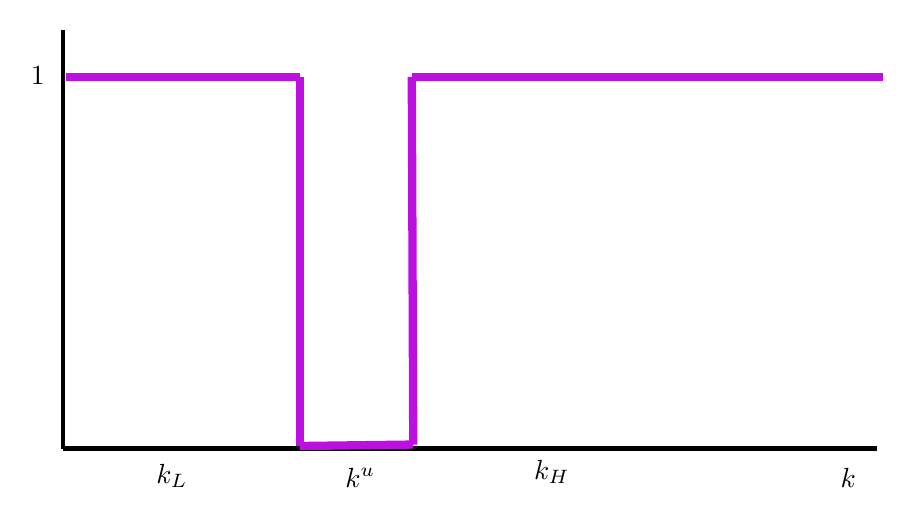
\begin{tikzpicture}[x=0.75pt,y=0.75pt,yscale=-0.7,xscale=0.7]
%uncomment if require: \path (0,365); %set diagram left start at 0, and has height of 365

%Straight Lines [id:da2969157887798486] 
\draw [line width=1.5]    (82.11,296.24) -- (642,296.24) ;
%Straight Lines [id:da8446473446760612] 
\draw [line width=1.5]    (82.11,8) -- (82.11,296.24) ;
%Straight Lines [id:da9938730496621584] 
\draw [color={rgb, 255:red, 189; green, 16; blue, 224 }  ,draw opacity=1 ][line width=3]    (245,40.5) -- (245,294.5) ;
%Straight Lines [id:da3902711000926453] 
\draw [color={rgb, 255:red, 189; green, 16; blue, 224 }  ,draw opacity=1 ][line width=3]    (322,40.5) -- (323,293.5) ;
%Straight Lines [id:da3078912288601936] 
\draw [color={rgb, 255:red, 189; green, 16; blue, 224 }  ,draw opacity=1 ][line width=3]    (245,40.5) -- (84,40.5) ;
%Straight Lines [id:da7102335211401436] 
\draw [color={rgb, 255:red, 189; green, 16; blue, 224 }  ,draw opacity=1 ][line width=3]    (646,40.5) -- (322,40.5) ;
%Straight Lines [id:da09422694839039836] 
\draw [color={rgb, 255:red, 189; green, 16; blue, 224 }  ,draw opacity=1 ][line width=3]    (323,293.5) -- (245,294.5) ;

% Text Node
\draw (615.27,307.69) node [anchor=north west][inner sep=0.75pt]    {$k$};
% Text Node
\draw (274.45,307.69) node [anchor=north west][inner sep=0.75pt]    {$k^{u}$};
% Text Node
\draw (144.45,305.4) node [anchor=north west][inner sep=0.75pt]    {$k_{L}$};
% Text Node
\draw (404.45,302.4) node [anchor=north west][inner sep=0.75pt]    {$k_{H}$};
% Text Node
\draw (58,31.4) node [anchor=north west][inner sep=0.75pt]    {$1$};
\end{tikzpicture}
\end{frame}

\begin{frame}{Variation in $\chi$}
Once we account for variation in $\chi$, the adjustment region is probabilistic.
$$\Omega(k,a) = \text{Prob}(V^a(k,a) - \chi w > V^n(k,a))$$
\end{frame}


\begin{frame}{Adjustment Hazard Function}


\tikzset{every picture/.style={line width=0.75pt}} %set default line width to 0.75pt        

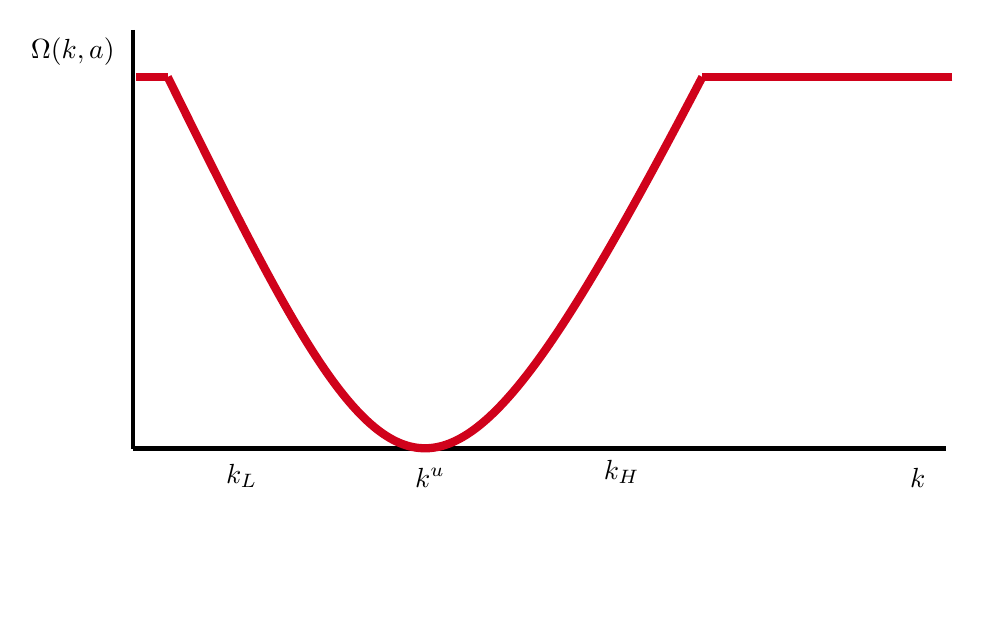
\begin{tikzpicture}[x=0.75pt,y=0.75pt,yscale=-0.7,xscale=0.7]

%Straight Lines [id:da672222002397836] 
\draw [line width=1.5]    (82.11,296.24) -- (642,296.24) ;
%Straight Lines [id:da7611775168579242] 
\draw [line width=1.5]    (82.11,8) -- (82.11,296.24) ;
%Straight Lines [id:da3612313886413103] 
\draw [color={rgb, 255:red, 208; green, 2; blue, 27 }  ,draw opacity=1 ][line width=3]    (106,40.5) -- (84,40.5) ;
%Straight Lines [id:da5733270980898113] 
\draw [color={rgb, 255:red, 208; green, 2; blue, 27 }  ,draw opacity=1 ][line width=3]    (646,40.5) -- (474,40.5) ;
%Curve Lines [id:da28941279963644084] 
\draw [color={rgb, 255:red, 208; green, 2; blue, 27 }  ,draw opacity=1 ][line width=3]    (106,40.5) .. controls (265,362.5) and (286,399.5) .. (474,40.5) ;

% Text Node
\draw (615.27,307.69) node [anchor=north west][inner sep=0.75pt]    {$k$};
% Text Node
\draw (274.45,307.69) node [anchor=north west][inner sep=0.75pt]    {$k^{u}$};
% Text Node
\draw (144.45,305.4) node [anchor=north west][inner sep=0.75pt]    {$k_{L}$};
% Text Node
\draw (404.45,302.4) node [anchor=north west][inner sep=0.75pt]    {$k_{H}$};
% Text Node
\draw (10,11.4) node [anchor=north west][inner sep=0.75pt]  [font=\normalsize]  {$\Omega ( k,a)$};


\end{tikzpicture}
\end{frame}

\begin{frame}{Back to the more general problem}
\begin{itemize}
\item I simulated for you the solution to the more general problem we considered before
\pause
\item I chose standard values for the parameters
\end{itemize}
\end{frame}

\begin{frame}{Value of Adjustment}
\begin{figure}
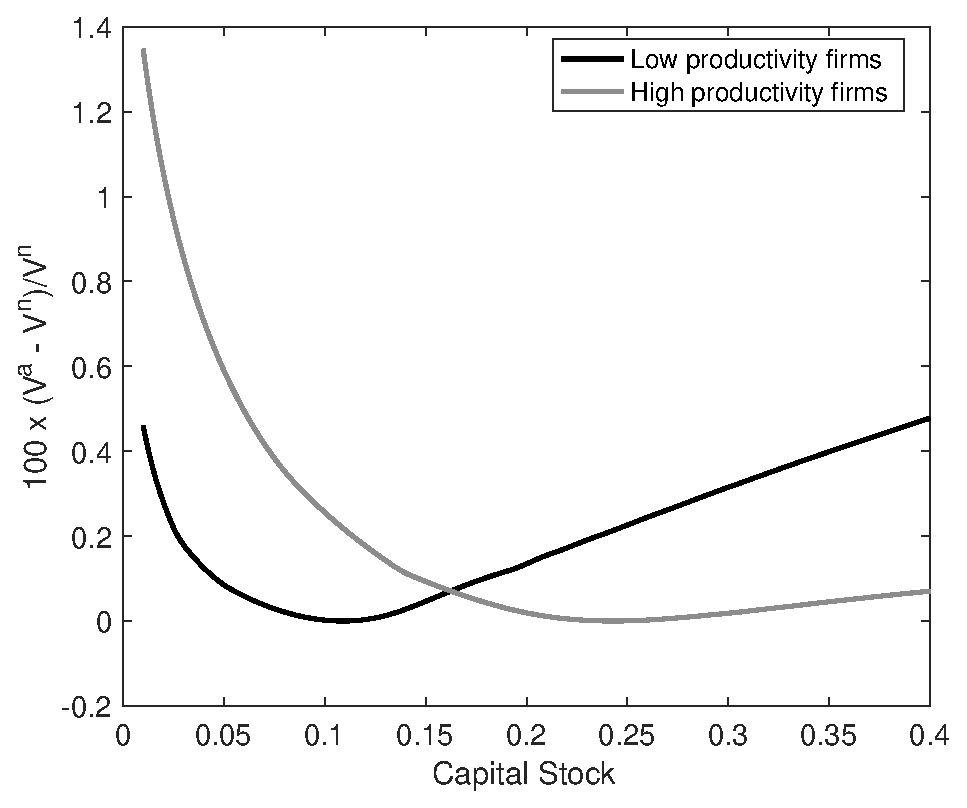
\includegraphics[scale=0.5]{FiguresTables/v_f.eps}
\end{figure}
\end{frame}

\begin{frame}{Adjustment Probability}
\begin{figure}
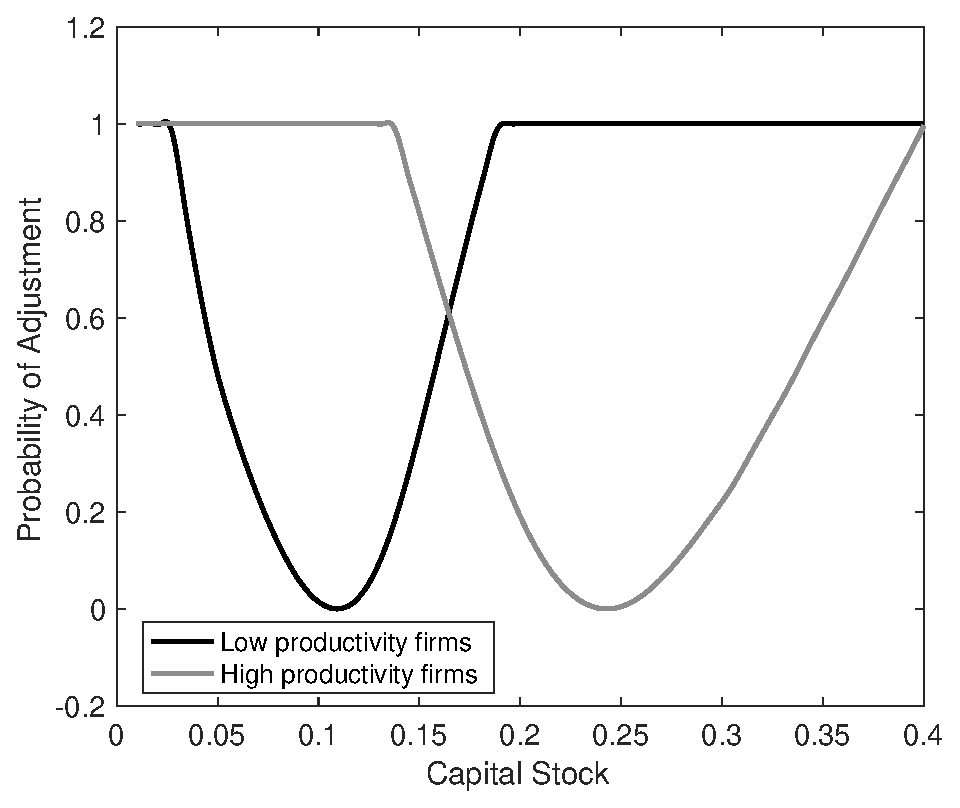
\includegraphics[scale=0.5]{FiguresTables/prob_adj.eps}
\end{figure}
\end{frame}


\begin{frame}{Cooper and Haltiwanger (2006)}
\begin{itemize}
\item That in a panel of firms $\psi$ and $\chi$ move different cross-sectional moments in different directions offers hope for a \textit{model-based} identification of this parameters
\pause
\begin{itemize}
\item Indirect evidence on the value of a parameter, given the predictions of a model about a moment, rather than direct evidence on an elasticity driven by a natural experiment
\end{itemize}
\pause
\item Use census data in order to estimate these cost of adjustment parameters
\end{itemize}
\end{frame}

\begin{frame}{Cooper and Haltiwanger 2006}
\begin{figure}
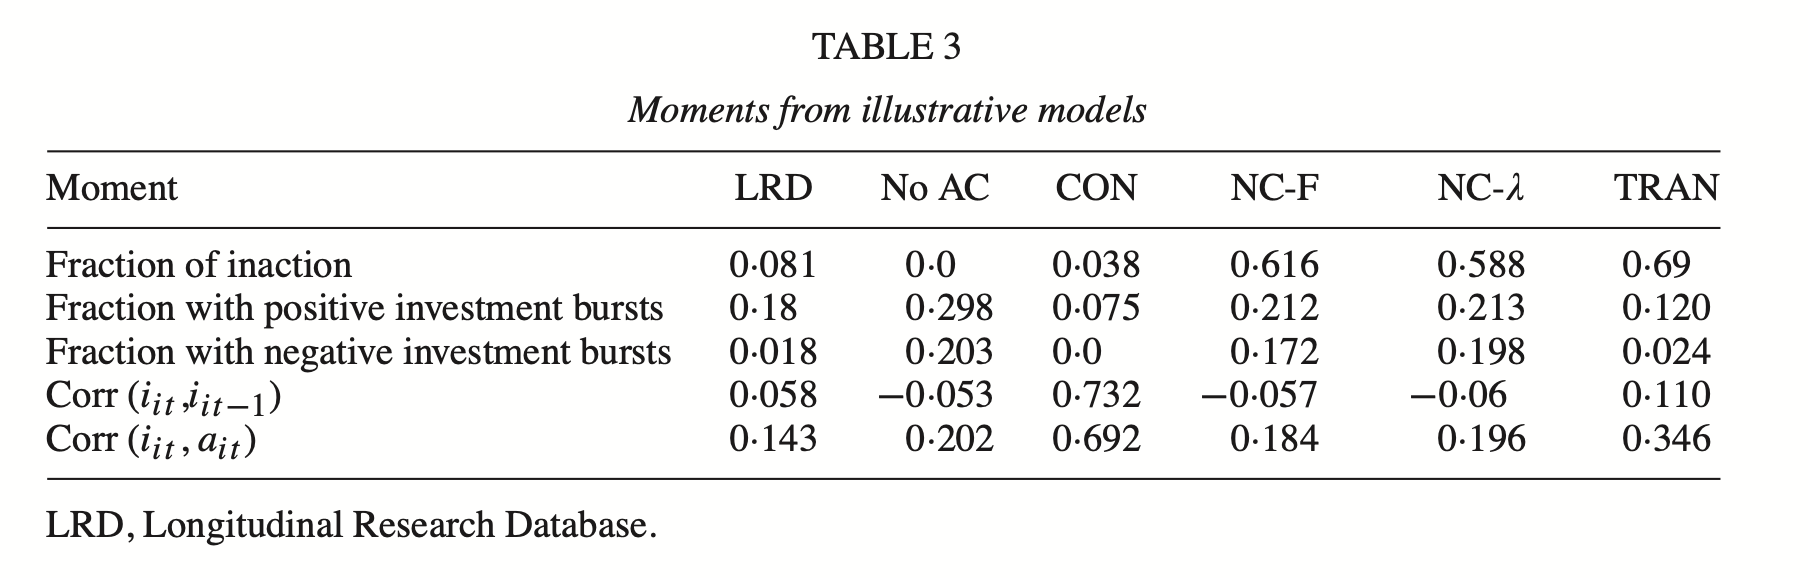
\includegraphics[scale=0.35]{FiguresTables/ch_1}
\end{figure}
LRD: Data. No AC: no adjustment costs. CON: convex costs. NC F: Fixed costs. NC $\lambda$: fixed drops in productivity during adjustment. $Tran$ Model of irreversibility.
\end{frame}

\begin{frame}{Cooper and Haltiwanger 2006}
\begin{figure}
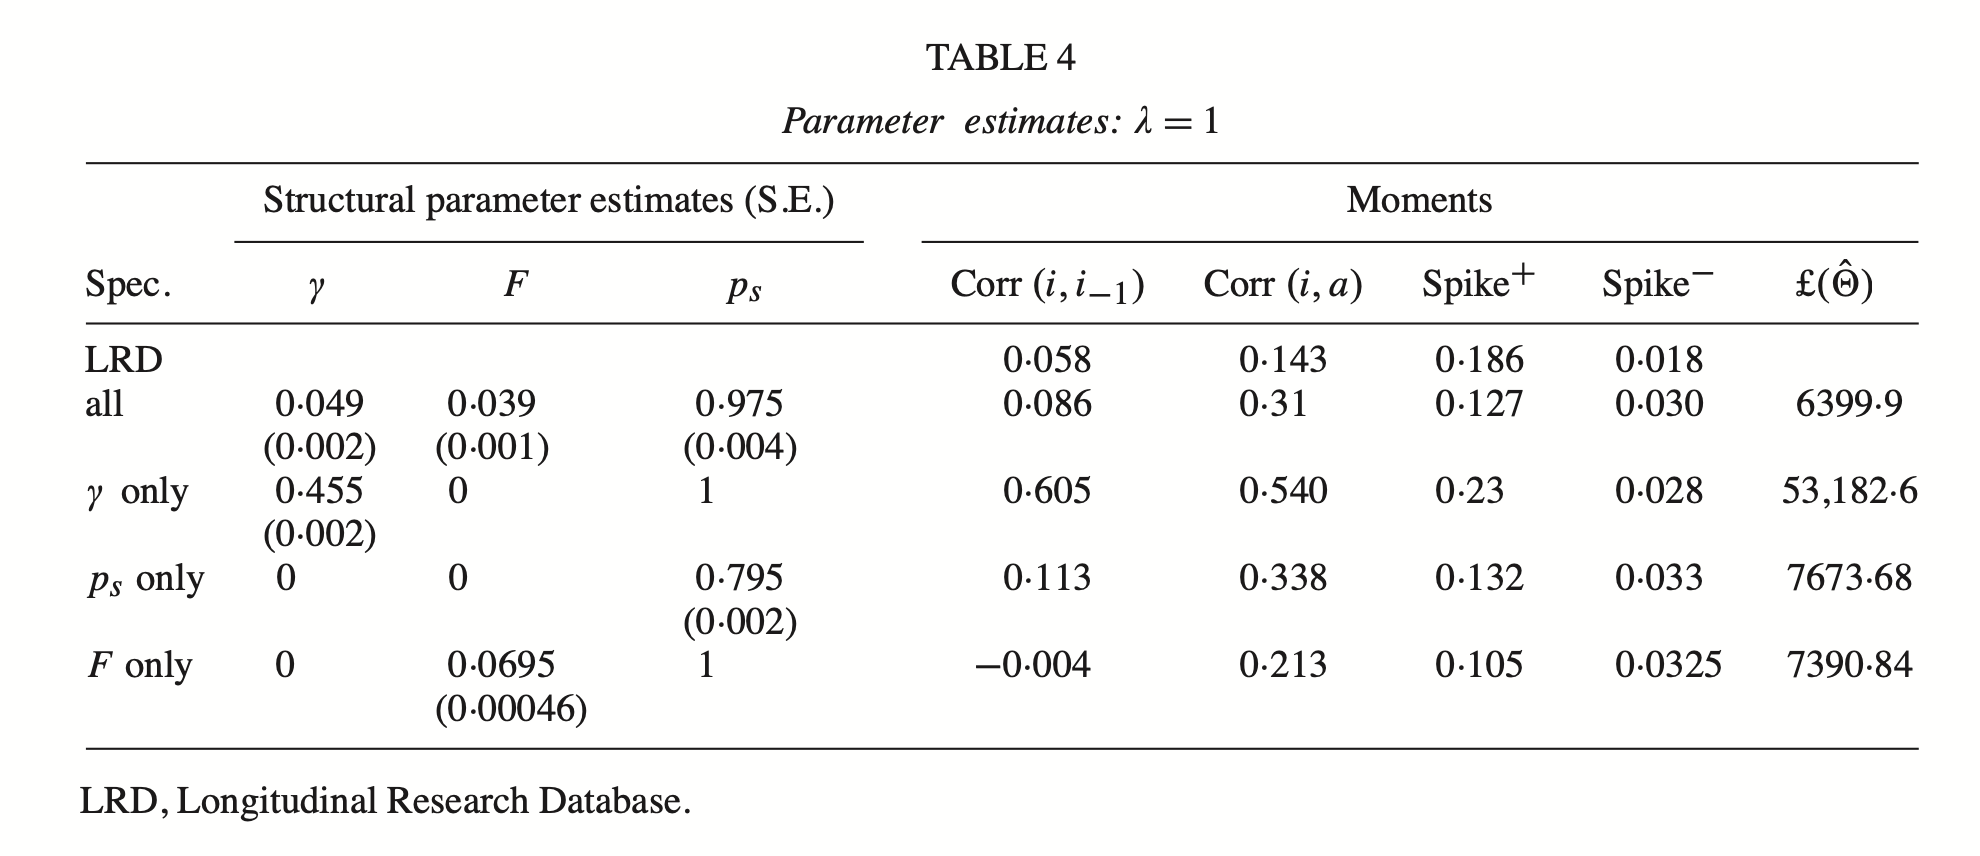
\includegraphics[scale=0.35]{FiguresTables/ch_2}
\end{figure}
$\gamma$: convex cost. $F$: fixed cost. $p_s$ transaction cost
\end{frame}
%	


\begin{frame}{Cooper and Haltiwanger 2006}
\begin{itemize}
\item Structural estimation
\item The model prefers a combination of costs
\end{itemize}
\end{frame}

\begin{frame}{Macro implications of micro adjustment}
\begin{itemize}
\item Caballero and Engel (1999) in a stripped down model show that one can summarize our problem as a function of disequilibrium capital $x$
\pause
\item In a setting a bit simpler than that of Caballero and Engel (1999) 
$$x_{jt} = \log k_{jt} - \log k^*_{jt}$$
\pause
\item where $k^*$ is the desired level of capital of a firm
\pause
\item Firms have adjustment probability $\Lambda(x)$
\pause
\item And conditional on adjustment they invest:
$k^* - k = \left(\frac{k^* - k}{k}\right) k = \left(\frac{k^*}{k} - 1 \right) k = (e^{-x} - 1)k$
\end{itemize}
\end{frame}



\begin{frame}{Caballero and Engel (1999)}
$$k^* - k = \left(\frac{k^* - k}{k}\right) k = \left(\frac{k^*}{k} - 1 \right) k = (e^{-x} - 1)k$$
\pause
\begin{itemize}
\item Average investment of firms with desiquilibrium $x$ is
$$\mathbb{E}_{\chi} \left[ I_{jt}(x) | x \right] = \Lambda(x)   (e^{-x} - 1)k(x)$$
\pause
\vspace{-0.5cm}
\item Integrating over firms
$$\frac{I_t^A}{K^A_t} \approx \int  (e^{-x} - 1)\Lambda(x)f(x,t) dx$$
\pause
\item where $f$ is the cross-sectional distribution of firms' capital disequilibrium at time $t$
\end{itemize}
\end{frame}

\begin{frame}{Caballero and Engel (1999)}
$$\frac{I_t^A}{K^A_t} \approx \int  (e^{-x} - 1)\Lambda(x)f(x,t) dx$$
\pause
\vspace{-0.5cm}
\begin{itemize}
\item To know aggregate investment one must know the \textit{cross-sectional distribution of disequilibrium}
\pause
\item It is \textit{not} sufficient to know the \textit{average disequilibrium} before adjustment.
\pause
\item As an alternative consider a model where $\Lambda(x) = 1$, and the mass of $f(x)$ is ``close to zero''
\pause
$$-x \approx \log(1-x)$$
\vspace{-0.5cm}
$$e^{-x} - 1 \approx - x$$
\vspace{-0.5cm}
\item and our expression becomes
$$\frac{I_t^A}{K^A_t} \approx \int -x f(x,t) dx = -X^A$$
\vspace{-0.5cm}
\item It \textbf{is} sufficient to know the \textit{average disequilibrium} before adjustment. 

\end{itemize}
\end{frame}

\begin{frame}{Aggregate Shocks}
\begin{itemize}
\item You should be uncomfortable seeing the title of this slide
\pause
\item This model is partial equilibrium. It does not have
\pause
\begin{itemize}
\item An endogenous wage rate
\pause
\item An endogenous real interest rate
\pause
\end{itemize}
\item An aggregate shock will move aggregate capital and labor demand
\pause
\item And $w$ and $r$ should move to clear markets
\pause
\item We are going to abstract from that for now
\pause
\item You can understand the results we will have as very short-run responses. Before prices adjust.
\end{itemize}
\end{frame}

\begin{frame}{Aggregate Shocks}
\begin{itemize}
\item With aggregate shocks
$$\frac{I_t^A}{K^A_t} \approx \int  (e^{-x} - 1)\Lambda(x)f(x+\delta + v_t ,t-1) dx$$
\item where $v_t$ is an aggregate shock
\pause
\item Depreciation increases imbalances, as do positive aggregate shocks
\pause
\item Ignoring changes in $w$ and $r$ imply that $\Lambda(.)$ is an invariant function
\end{itemize}
\end{frame}


\begin{frame}{State dependence}
\centering

\tikzset{every picture/.style={line width=0.75pt}} %set default line width to 0.75pt        

\begin{tikzpicture}[x=0.75pt,y=0.75pt,yscale=-1,xscale=1]
%uncomment if require: \path (0,300); %set diagram left start at 0, and has height of 300

%Straight Lines [id:da7539706503095034] 
\draw    (134,215) -- (481,215) ;
\draw [shift={(483,215)}, rotate = 180] [color={rgb, 255:red, 0; green, 0; blue, 0 }  ][line width=0.75]    (10.93,-3.29) .. controls (6.95,-1.4) and (3.31,-0.3) .. (0,0) .. controls (3.31,0.3) and (6.95,1.4) .. (10.93,3.29)   ;
%Straight Lines [id:da24902826661718125] 
\draw    (134,215) -- (134,29) ;
\draw [shift={(134,27)}, rotate = 90] [color={rgb, 255:red, 0; green, 0; blue, 0 }  ][line width=0.75]    (10.93,-3.29) .. controls (6.95,-1.4) and (3.31,-0.3) .. (0,0) .. controls (3.31,0.3) and (6.95,1.4) .. (10.93,3.29)   ;
%Straight Lines [id:da1863368412726374] 
\draw [color={rgb, 255:red, 208; green, 2; blue, 27 }  ,draw opacity=1 ]   (134,66) -- (210,66) ;
%Straight Lines [id:da9241783388704874] 
\draw [color={rgb, 255:red, 208; green, 2; blue, 27 }  ,draw opacity=1 ]   (210,66) -- (210,216) ;
%Straight Lines [id:da359650145377848] 
\draw [color={rgb, 255:red, 208; green, 2; blue, 27 }  ,draw opacity=1 ]   (397,66) -- (397,216) ;
%Straight Lines [id:da541627462790579] 
\draw [color={rgb, 255:red, 208; green, 2; blue, 27 }  ,draw opacity=1 ]   (397,66) -- (485,66) ;
%Straight Lines [id:da8885401430722457] 
\draw [color={rgb, 255:red, 208; green, 2; blue, 27 }  ,draw opacity=1 ]   (210,216) -- (397,216) ;
%Curve Lines [id:da7607396145235965] 
\draw    (236,213) .. controls (318,227) and (288,68) .. (304,67) .. controls (320,66) and (295,227) .. (364,214) ;
%Straight Lines [id:da7641693782495453] 
\draw  [dash pattern={on 4.5pt off 4.5pt}]  (303.5,7) -- (303.5,216) ;

% Text Node
\draw (449,231.4) node [anchor=north west][inner sep=0.75pt]    {$x\ =\ k^{*} \ -\ k$};
% Text Node
\draw (112,56.4) node [anchor=north west][inner sep=0.75pt]    {$1$};
% Text Node
\draw (166,41.4) node [anchor=north west][inner sep=0.75pt]  [color={rgb, 255:red, 208; green, 2; blue, 27 }  ,opacity=1 ]  {$\Omega ( x)$};
% Text Node
\draw (314,46.4) node [anchor=north west][inner sep=0.75pt]  [color={rgb, 255:red, 0; green, 0; blue, 0 }  ,opacity=1 ]  {$f( x)$};
% Text Node
\draw (295,221.4) node [anchor=north west][inner sep=0.75pt]    {$0$};


\end{tikzpicture}
\end{frame}


\begin{frame}{State dependence}
\centering

\tikzset{every picture/.style={line width=0.75pt}} %set default line width to 0.75pt        

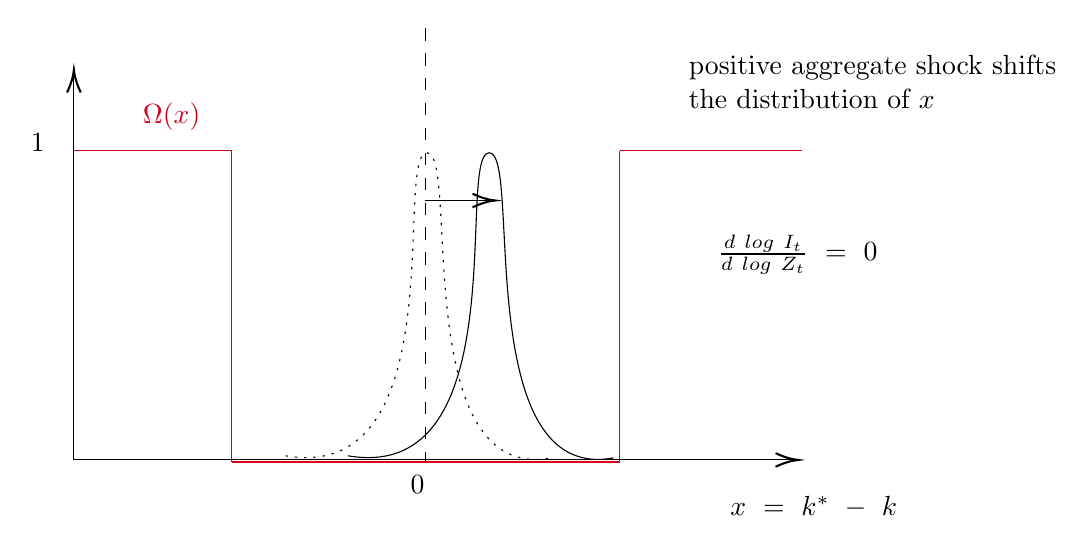
\begin{tikzpicture}[x=0.75pt,y=0.75pt,yscale=-1,xscale=1]
%uncomment if require: \path (0,300); %set diagram left start at 0, and has height of 300

%Straight Lines [id:da9155815042462783] 
\draw    (134,215) -- (481,215) ;
\draw [shift={(483,215)}, rotate = 180] [color={rgb, 255:red, 0; green, 0; blue, 0 }  ][line width=0.75]    (10.93,-3.29) .. controls (6.95,-1.4) and (3.31,-0.3) .. (0,0) .. controls (3.31,0.3) and (6.95,1.4) .. (10.93,3.29)   ;
%Straight Lines [id:da4129992859383682] 
\draw    (134,215) -- (134,29) ;
\draw [shift={(134,27)}, rotate = 90] [color={rgb, 255:red, 0; green, 0; blue, 0 }  ][line width=0.75]    (10.93,-3.29) .. controls (6.95,-1.4) and (3.31,-0.3) .. (0,0) .. controls (3.31,0.3) and (6.95,1.4) .. (10.93,3.29)   ;
%Straight Lines [id:da4371652510955124] 
\draw [color={rgb, 255:red, 208; green, 2; blue, 27 }  ,draw opacity=1 ]   (134,66) -- (210,66) ;
%Straight Lines [id:da019650341636526125] 
\draw [color={rgb, 255:red, 208; green, 2; blue, 27 }  ,draw opacity=1 ]   (210,66) -- (210,216) ;
%Straight Lines [id:da771002255172021] 
\draw [color={rgb, 255:red, 208; green, 2; blue, 27 }  ,draw opacity=1 ]   (397,66) -- (397,216) ;
%Straight Lines [id:da9123354153291034] 
\draw [color={rgb, 255:red, 208; green, 2; blue, 27 }  ,draw opacity=1 ]   (397,66) -- (485,66) ;
%Straight Lines [id:da7860051271727608] 
\draw [color={rgb, 255:red, 208; green, 2; blue, 27 }  ,draw opacity=1 ]   (210,216) -- (397,216) ;
%Curve Lines [id:da8344985195886927] 
\draw  [dash pattern={on 0.84pt off 2.51pt}]  (236,213) .. controls (318,227) and (288,68) .. (304,67) .. controls (320,66) and (295,227) .. (364,214) ;
%Straight Lines [id:da6021947296093324] 
\draw  [dash pattern={on 4.5pt off 4.5pt}]  (303.5,7) -- (303.5,216) ;
%Curve Lines [id:da5687728525234115] 
\draw    (266,213) .. controls (348,227) and (318,68) .. (334,67) .. controls (350,66) and (325,227) .. (394,214) ;
%Straight Lines [id:da06100422083096735] 
\draw    (303,90) -- (335,90) ;
\draw [shift={(337,90)}, rotate = 180] [color={rgb, 255:red, 0; green, 0; blue, 0 }  ][line width=0.75]    (10.93,-3.29) .. controls (6.95,-1.4) and (3.31,-0.3) .. (0,0) .. controls (3.31,0.3) and (6.95,1.4) .. (10.93,3.29)   ;

% Text Node
\draw (449,231.4) node [anchor=north west][inner sep=0.75pt]    {$x\ =\ k^{*} \ -\ k$};
% Text Node
\draw (112,56.4) node [anchor=north west][inner sep=0.75pt]    {$1$};
% Text Node
\draw (166,41.4) node [anchor=north west][inner sep=0.75pt]  [color={rgb, 255:red, 208; green, 2; blue, 27 }  ,opacity=1 ]  {$\Omega ( x)$};
% Text Node
\draw (295,221.4) node [anchor=north west][inner sep=0.75pt]    {$0$};
% Text Node
\draw (429,19) node [anchor=north west][inner sep=0.75pt]   [align=left] {positive aggregate shock shifts\\the distribution of $\displaystyle x$};
% Text Node
\draw (443,105.4) node [anchor=north west][inner sep=0.75pt]    {$\frac{d\ log\ I_{t}}{d\ log\ Z_{t}} \ =\ 0$};


\end{tikzpicture}
\end{frame}


\begin{frame}{State Dependence}
\centering
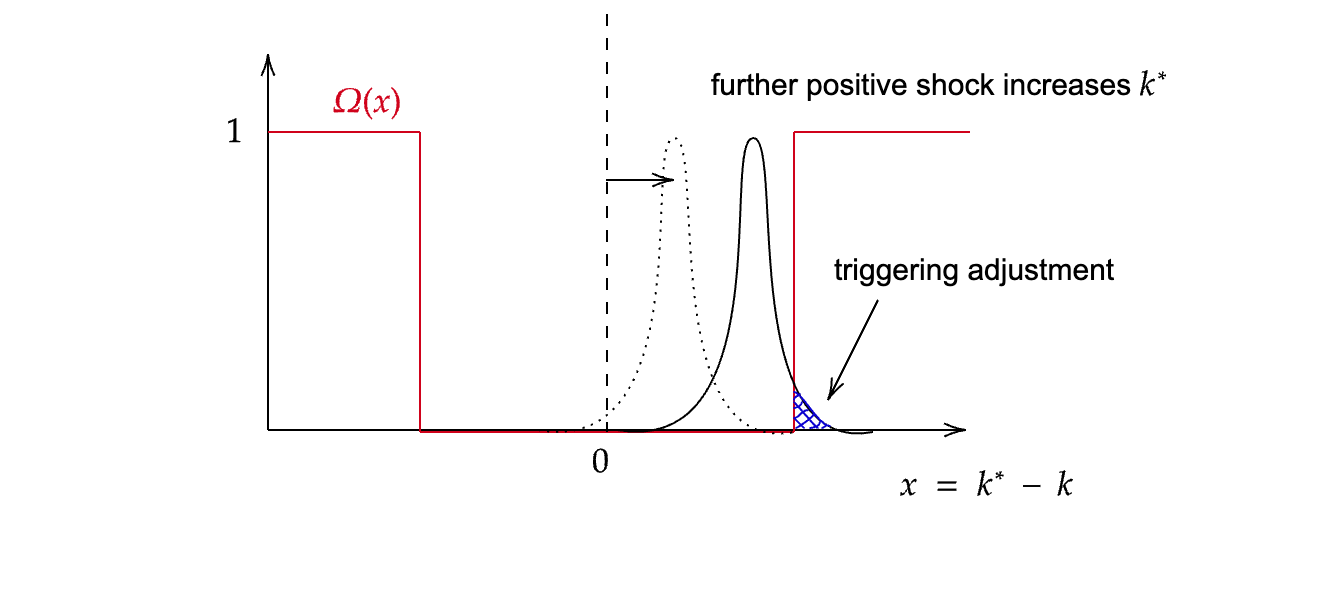
\includegraphics[scale=0.3]{FiguresTables/st_dep_3}
\end{frame}


\begin{frame}{State Dependence}
\centering
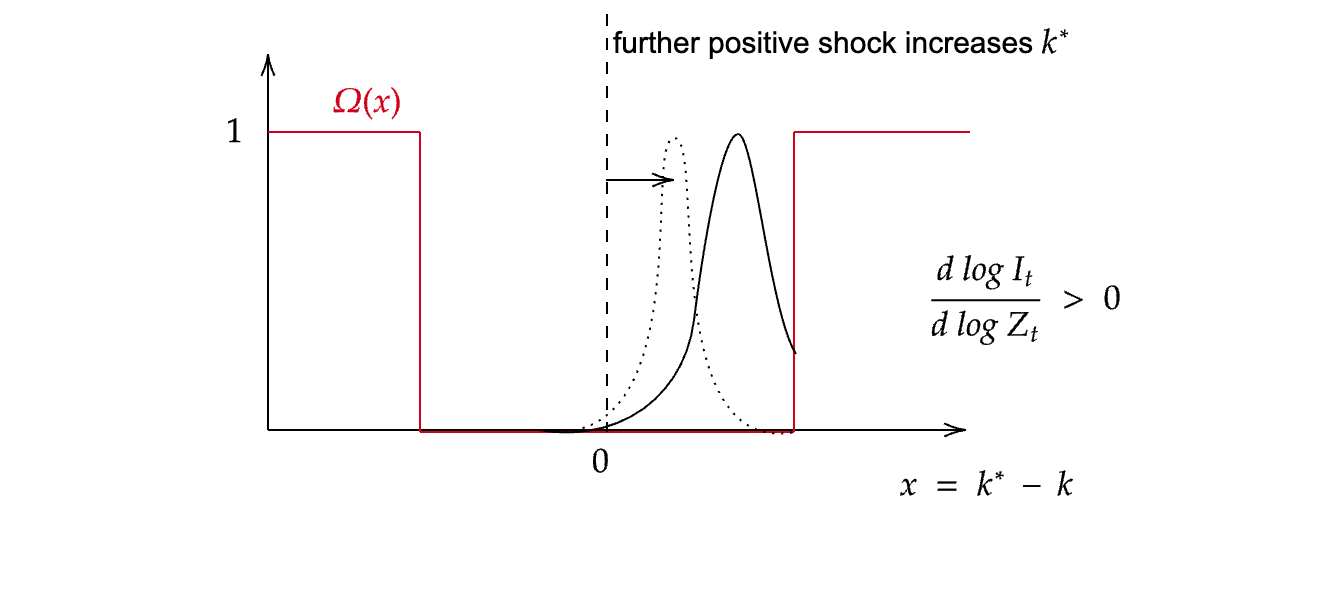
\includegraphics[scale=0.3]{FiguresTables/st_dep_4}
\end{frame}


\begin{frame}{State Dependence}
\centering
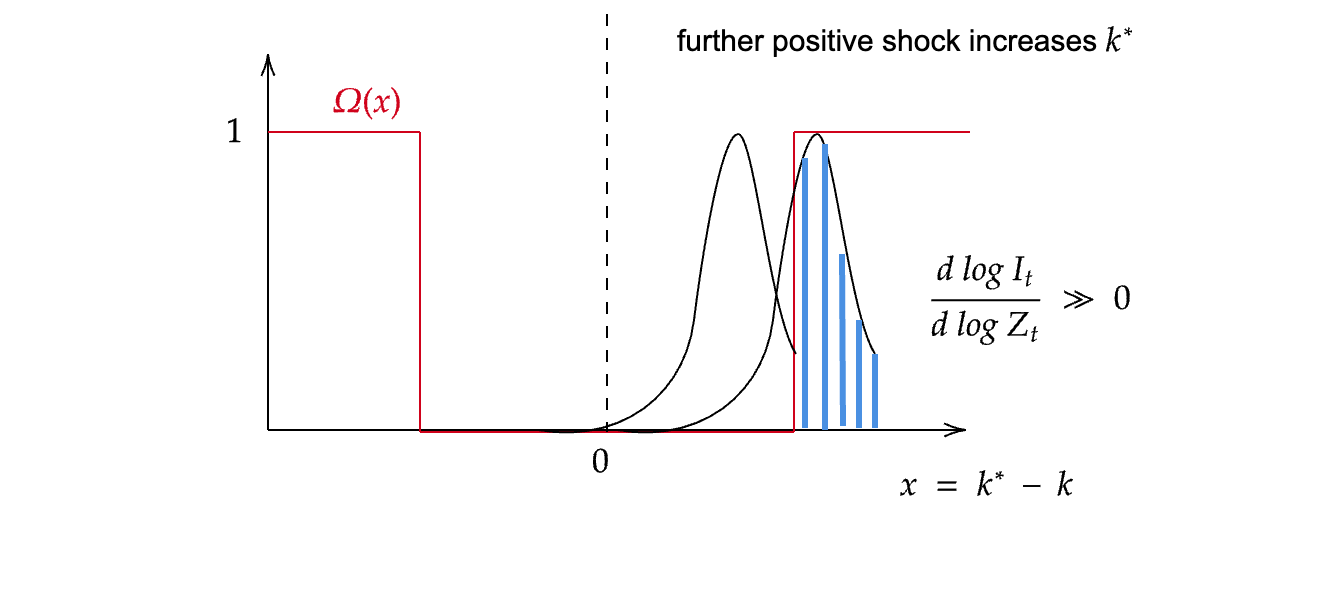
\includegraphics[scale=0.3]{FiguresTables/st_dep_5}
\end{frame}



\begin{frame}{Pent-Up Demand}
\begin{itemize}
\item Aggregate investment depends on the mass of firms that are \textit{close-enough} to adjustment
\pause
\item Therefore shocks of the same size may have differential effects on investment
\item As a function of the distribution of capital imbalances
\item Which means that the \textit{elasticity} of investment to an aggregate shock is state dependent
\item as in: it depends on the distribution of the state variables of the model
\item Remember your RBC model from 210A. Model is linear in logs. The elasticity of investment to a shock is invariant. Not guaranteed with fixed costs.
\end{itemize}
\end{frame}

\begin{frame}{Applications to Recessions and Recoveries}
\begin{itemize}
\item During a recession firms have ``excess capital''
\item Imagine a tax subsidy that makes positive investment cheaper
\item If no firm is near the threshold, then the reform is ineffective
\item Imagine a tax subsidy during a recovery
\item If the mass of firms that would have adjusted in the absence of the subsidy is large...
\item The reform subsidizes inframarginal firms, making tax subsidies more expensive per unit of investment
\end{itemize}
\end{frame}

\begin{frame}{Caballero Engel (1999)}
\begin{figure}
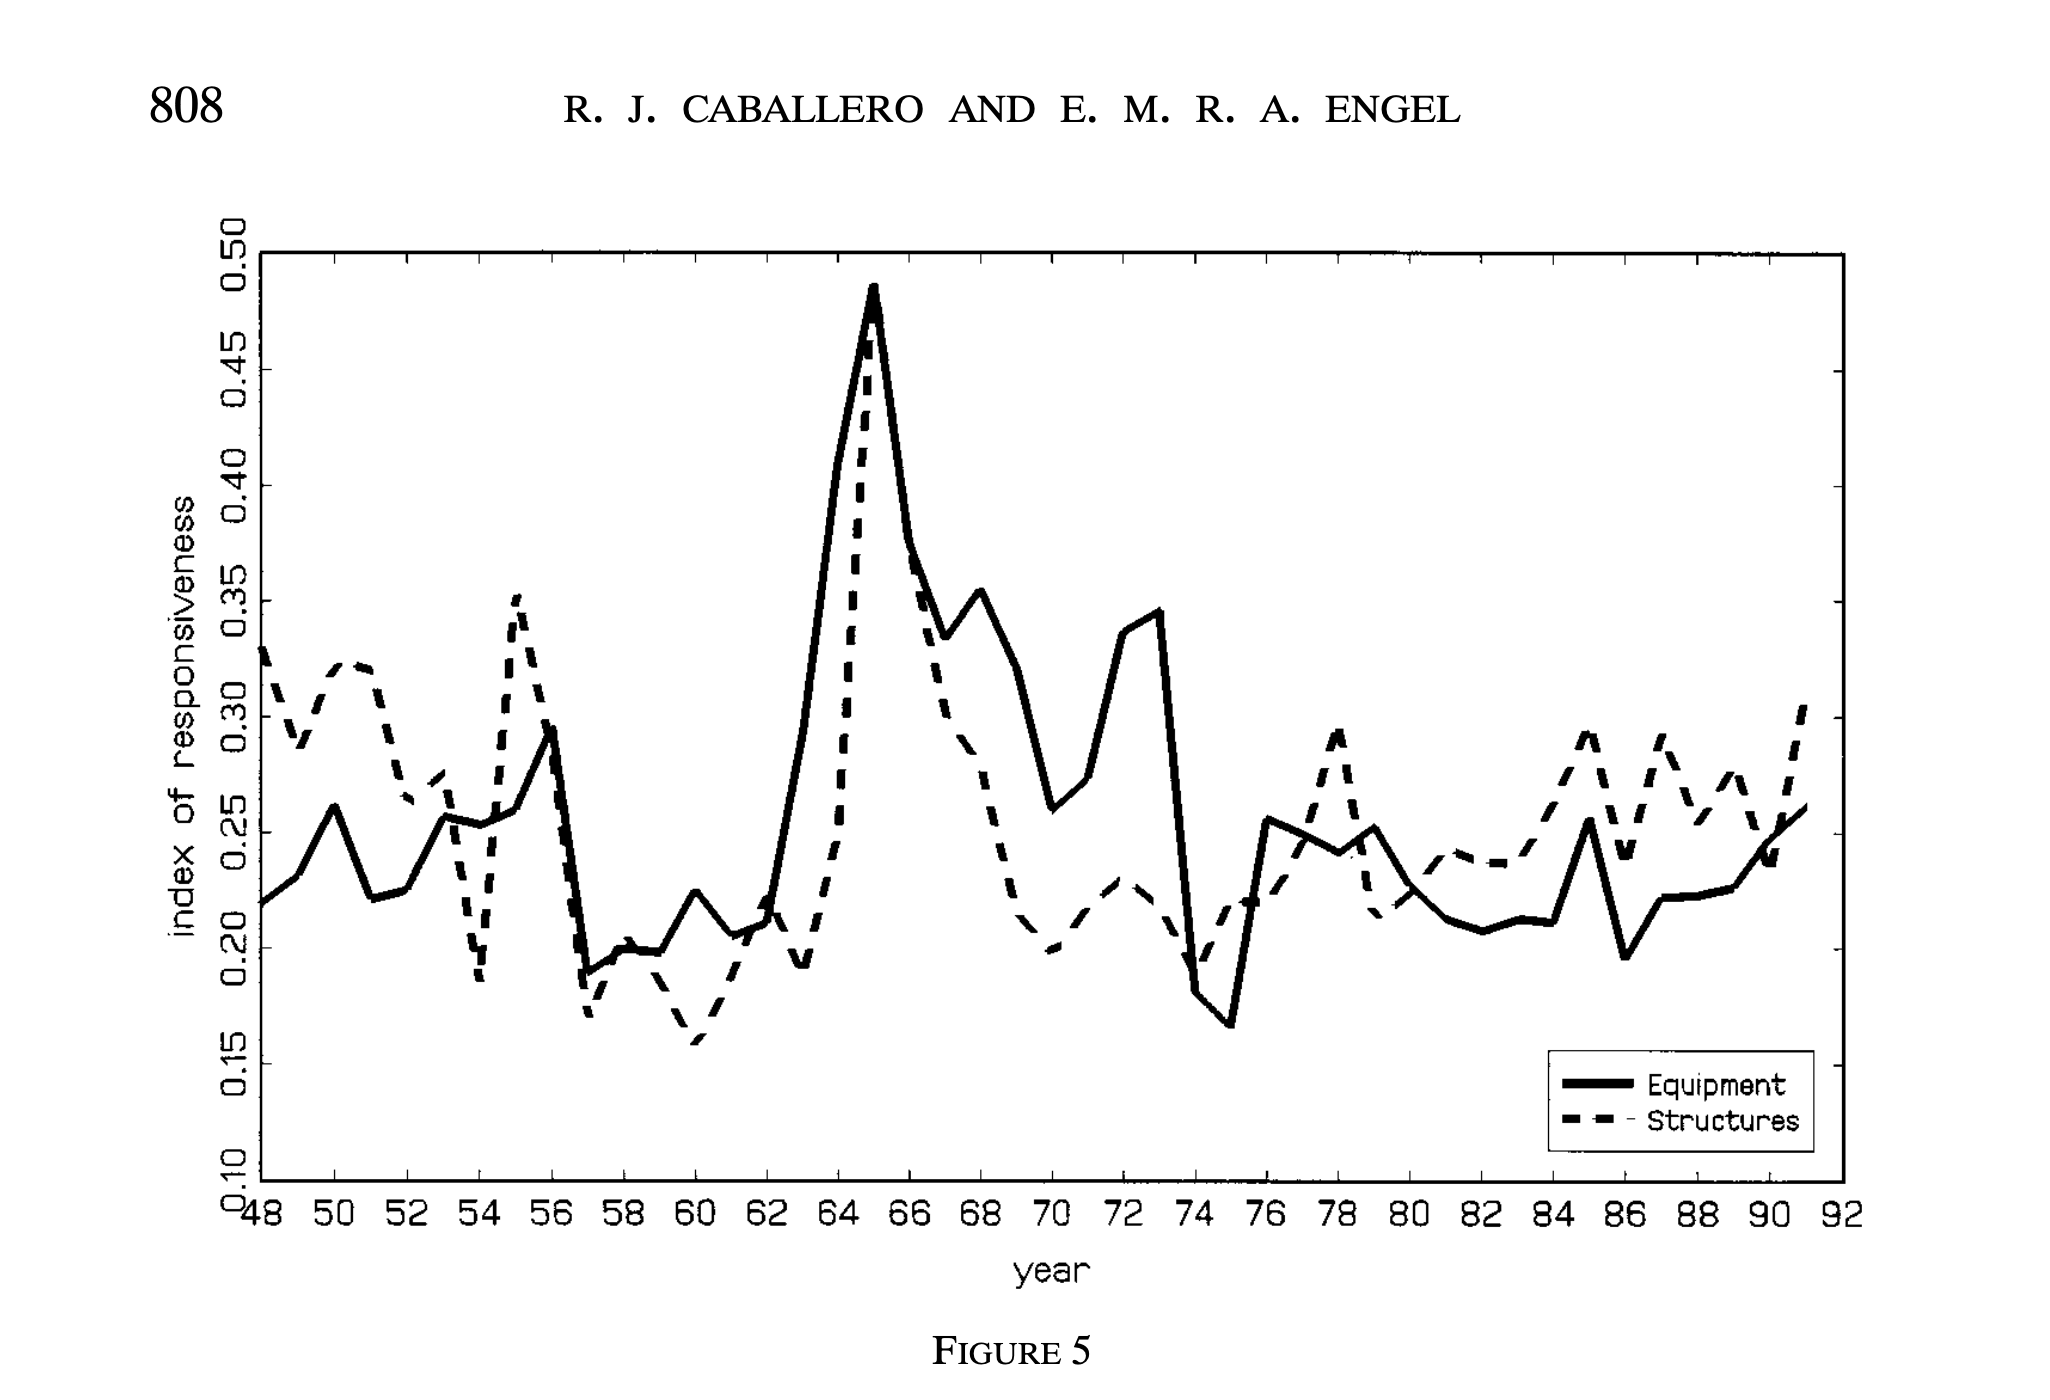
\includegraphics[scale=0.3]{FiguresTables/ch_3}
\end{figure}
The sensitivity of investment to additional shocks is time-varying
\end{frame}
\end{document}






